% Options for packages loaded elsewhere
\PassOptionsToPackage{unicode}{hyperref}
\PassOptionsToPackage{hyphens}{url}
%
\documentclass[
]{article}
\title{P8106 - Final Project - NBA Players Salary Prediction}
\author{Mingkuan Xu (mx2262), Mengfan Luo (ml4701), Yiqun Jin (yj2686)}
\date{05/11/2022}

\usepackage{amsmath,amssymb}
\usepackage{lmodern}
\usepackage{iftex}
\ifPDFTeX
  \usepackage[T1]{fontenc}
  \usepackage[utf8]{inputenc}
  \usepackage{textcomp} % provide euro and other symbols
\else % if luatex or xetex
  \usepackage{unicode-math}
  \defaultfontfeatures{Scale=MatchLowercase}
  \defaultfontfeatures[\rmfamily]{Ligatures=TeX,Scale=1}
\fi
% Use upquote if available, for straight quotes in verbatim environments
\IfFileExists{upquote.sty}{\usepackage{upquote}}{}
\IfFileExists{microtype.sty}{% use microtype if available
  \usepackage[]{microtype}
  \UseMicrotypeSet[protrusion]{basicmath} % disable protrusion for tt fonts
}{}
\makeatletter
\@ifundefined{KOMAClassName}{% if non-KOMA class
  \IfFileExists{parskip.sty}{%
    \usepackage{parskip}
  }{% else
    \setlength{\parindent}{0pt}
    \setlength{\parskip}{6pt plus 2pt minus 1pt}}
}{% if KOMA class
  \KOMAoptions{parskip=half}}
\makeatother
\usepackage{xcolor}
\IfFileExists{xurl.sty}{\usepackage{xurl}}{} % add URL line breaks if available
\IfFileExists{bookmark.sty}{\usepackage{bookmark}}{\usepackage{hyperref}}
\hypersetup{
  pdftitle={P8106 - Final Project - NBA Players Salary Prediction},
  pdfauthor={Mingkuan Xu (mx2262), Mengfan Luo (ml4701), Yiqun Jin (yj2686)},
  hidelinks,
  pdfcreator={LaTeX via pandoc}}
\urlstyle{same} % disable monospaced font for URLs
\usepackage[margin=1in]{geometry}
\usepackage{longtable,booktabs,array}
\usepackage{calc} % for calculating minipage widths
% Correct order of tables after \paragraph or \subparagraph
\usepackage{etoolbox}
\makeatletter
\patchcmd\longtable{\par}{\if@noskipsec\mbox{}\fi\par}{}{}
\makeatother
% Allow footnotes in longtable head/foot
\IfFileExists{footnotehyper.sty}{\usepackage{footnotehyper}}{\usepackage{footnote}}
\makesavenoteenv{longtable}
\usepackage{graphicx}
\makeatletter
\def\maxwidth{\ifdim\Gin@nat@width>\linewidth\linewidth\else\Gin@nat@width\fi}
\def\maxheight{\ifdim\Gin@nat@height>\textheight\textheight\else\Gin@nat@height\fi}
\makeatother
% Scale images if necessary, so that they will not overflow the page
% margins by default, and it is still possible to overwrite the defaults
% using explicit options in \includegraphics[width, height, ...]{}
\setkeys{Gin}{width=\maxwidth,height=\maxheight,keepaspectratio}
% Set default figure placement to htbp
\makeatletter
\def\fps@figure{htbp}
\makeatother
\setlength{\emergencystretch}{3em} % prevent overfull lines
\providecommand{\tightlist}{%
  \setlength{\itemsep}{0pt}\setlength{\parskip}{0pt}}
\setcounter{secnumdepth}{-\maxdimen} % remove section numbering
\ifLuaTeX
  \usepackage{selnolig}  % disable illegal ligatures
\fi

\begin{document}
\maketitle

\hypertarget{introduction}{%
\subsection{Introduction}\label{introduction}}

For teams in the National Basketball Association (NBA), a key strategy
to win more games is to properly allocate their salary cap - an
agreement that places a limit on the amount of money that a team can
spend on players' salaries. How to evaluate the performance of each NBA
player and give a suitable level of salary is a complicated problem. In
this project, we intend to predict the salary of NBA players in the
2021-2022 season based on their game statistics. We collected game
statistics that are commonly used to evaluate players from the NBA
official website, built linear, generalized linear, tree-based, and
neural network, and conducted model comparison to determine a final
predictive model.

\hypertarget{data-preprocessing}{%
\subsection{Data Preprocessing}\label{data-preprocessing}}

The data used for exploratory analysis and model construction are based
on two datasets: the NBA players' contracted salary dataset {[}1{]} and
game performance statistics dataset {[}2{]} in 2021-2022. The data were
preprocessed using the following pipeline:

\begin{itemize}
\tightlist
\item
  Two original datasets were inner joined by players and teams
\item
  Kept only one record with most number of games played for each of
  players, given a player may transfer to other teams during the session
  and have multiple records.
\item
  Removed 5 variables with missing values caused by division of other
  existing variables.
\item
  Divided count variables (\texttt{field\_goal}, \texttt{free\_throw},
  etc.) by variable \texttt{minute} to convert them to efficiency.
\end{itemize}

The final cleaned dataset contained 442 records and 24 variables,
including 2 categorical variables, 21 numerical variables and 1 numeric
response variable \texttt{salary} (Table 1).

\begin{longtable}[]{@{}lll@{}}
\caption{Table of Variables}\tabularnewline
\toprule
Variable Name & Meaning & Variable Type \\
\midrule
\endfirsthead
\toprule
Variable Name & Meaning & Variable Type \\
\midrule
\endhead
position & Position of the player & categorical (5 classes) \\
age & Player's age on February 1 of the season & numeric \\
team & Team that the player belong to & categorical (30 classes) \\
game & Number of games played & numeric \\
game\_starting & Number of games played as a starter & numeric \\
minute & Minutes played per game & numeric \\
field\_goal & Field goals per minute & numeric \\
fg\_attempt & Field goal attempts per minute & numeric \\
x3p & 3-point field goals per minute & numeric \\
x3p\_attempt & 3-point field goal attempts per minute & numeric \\
x2p & 2-point field goals per minute & numeric \\
x2p\_attempt & 2-point field goal attempts per minute & numeric \\
free\_throw & Free throws per minute & numeric \\
ft\_attempt & Free throw attempts per minute & numeric \\
offensive\_rb & Offensive rebounds per minute & numeric \\
defenssive\_rb & Defensive rebounds per minute & numeric \\
total\_rb & Total rebounds per minute & numeric \\
assistance & Assists per minute & numeric \\
steal & Steals per minute & numeric \\
block & Blocks per minute & numeric \\
turnover & Turnovers per minute & numeric \\
personal\_foul & Personal fouls per minute & numeric \\
point & Points per minute & numeric \\
salary & Salary of the player in million (Response) & numeric \\
\bottomrule
\end{longtable}

\hypertarget{exploratory-analysis}{%
\subsection{Exploratory Analysis}\label{exploratory-analysis}}

\hypertarget{univariate-analysis}{%
\subsubsection{Univariate Analysis}\label{univariate-analysis}}

The distribution of each variable in the dataset was plotted and
examined (Appendix A Figure 6\&7). Categorical variables \texttt{team}
and \texttt{position} were distributed quite evenly (Appendix A Figure
7). While 30 unique values in \texttt{team} might lead to too many dummy
variables in the model, the variable was considered to be excluded or
clustered into fewer classes for model fitting. For numeric variables,
some of them (\texttt{game\_starting}, \texttt{free\_throw},
\texttt{offenssive\_rb},\texttt{block}), including response
\texttt{salary} are skewed, with some players have extremely high
salary.

\hypertarget{correlation-analysis}{%
\subsubsection{Correlation Analysis}\label{correlation-analysis}}

From the correlation heatmap (Figure 1A), some variables were found to
be strongly correlated with others, leading to a potential problem of
multicolinearity. Such problem could be handled by using penalized
models (such as ridge/lasso regression and elastic-net) or ensembled
models (such as random forest, boosting, and neural network). From the
feature maps (Appendix A Figure 8), some predictive variables were found
to have non-linear correlations with \texttt{salary}, such as
\texttt{age}, \texttt{game}, \texttt{game\_starting},
\texttt{free\_throw}, \texttt{personal\_foul} and \texttt{point} (Figure
1B). Generalized linear regression models and other non-linear models,
including GAM, MARS, random forest and neural network model, could be
used to capture such non-linearity.

\begin{figure}
\centering
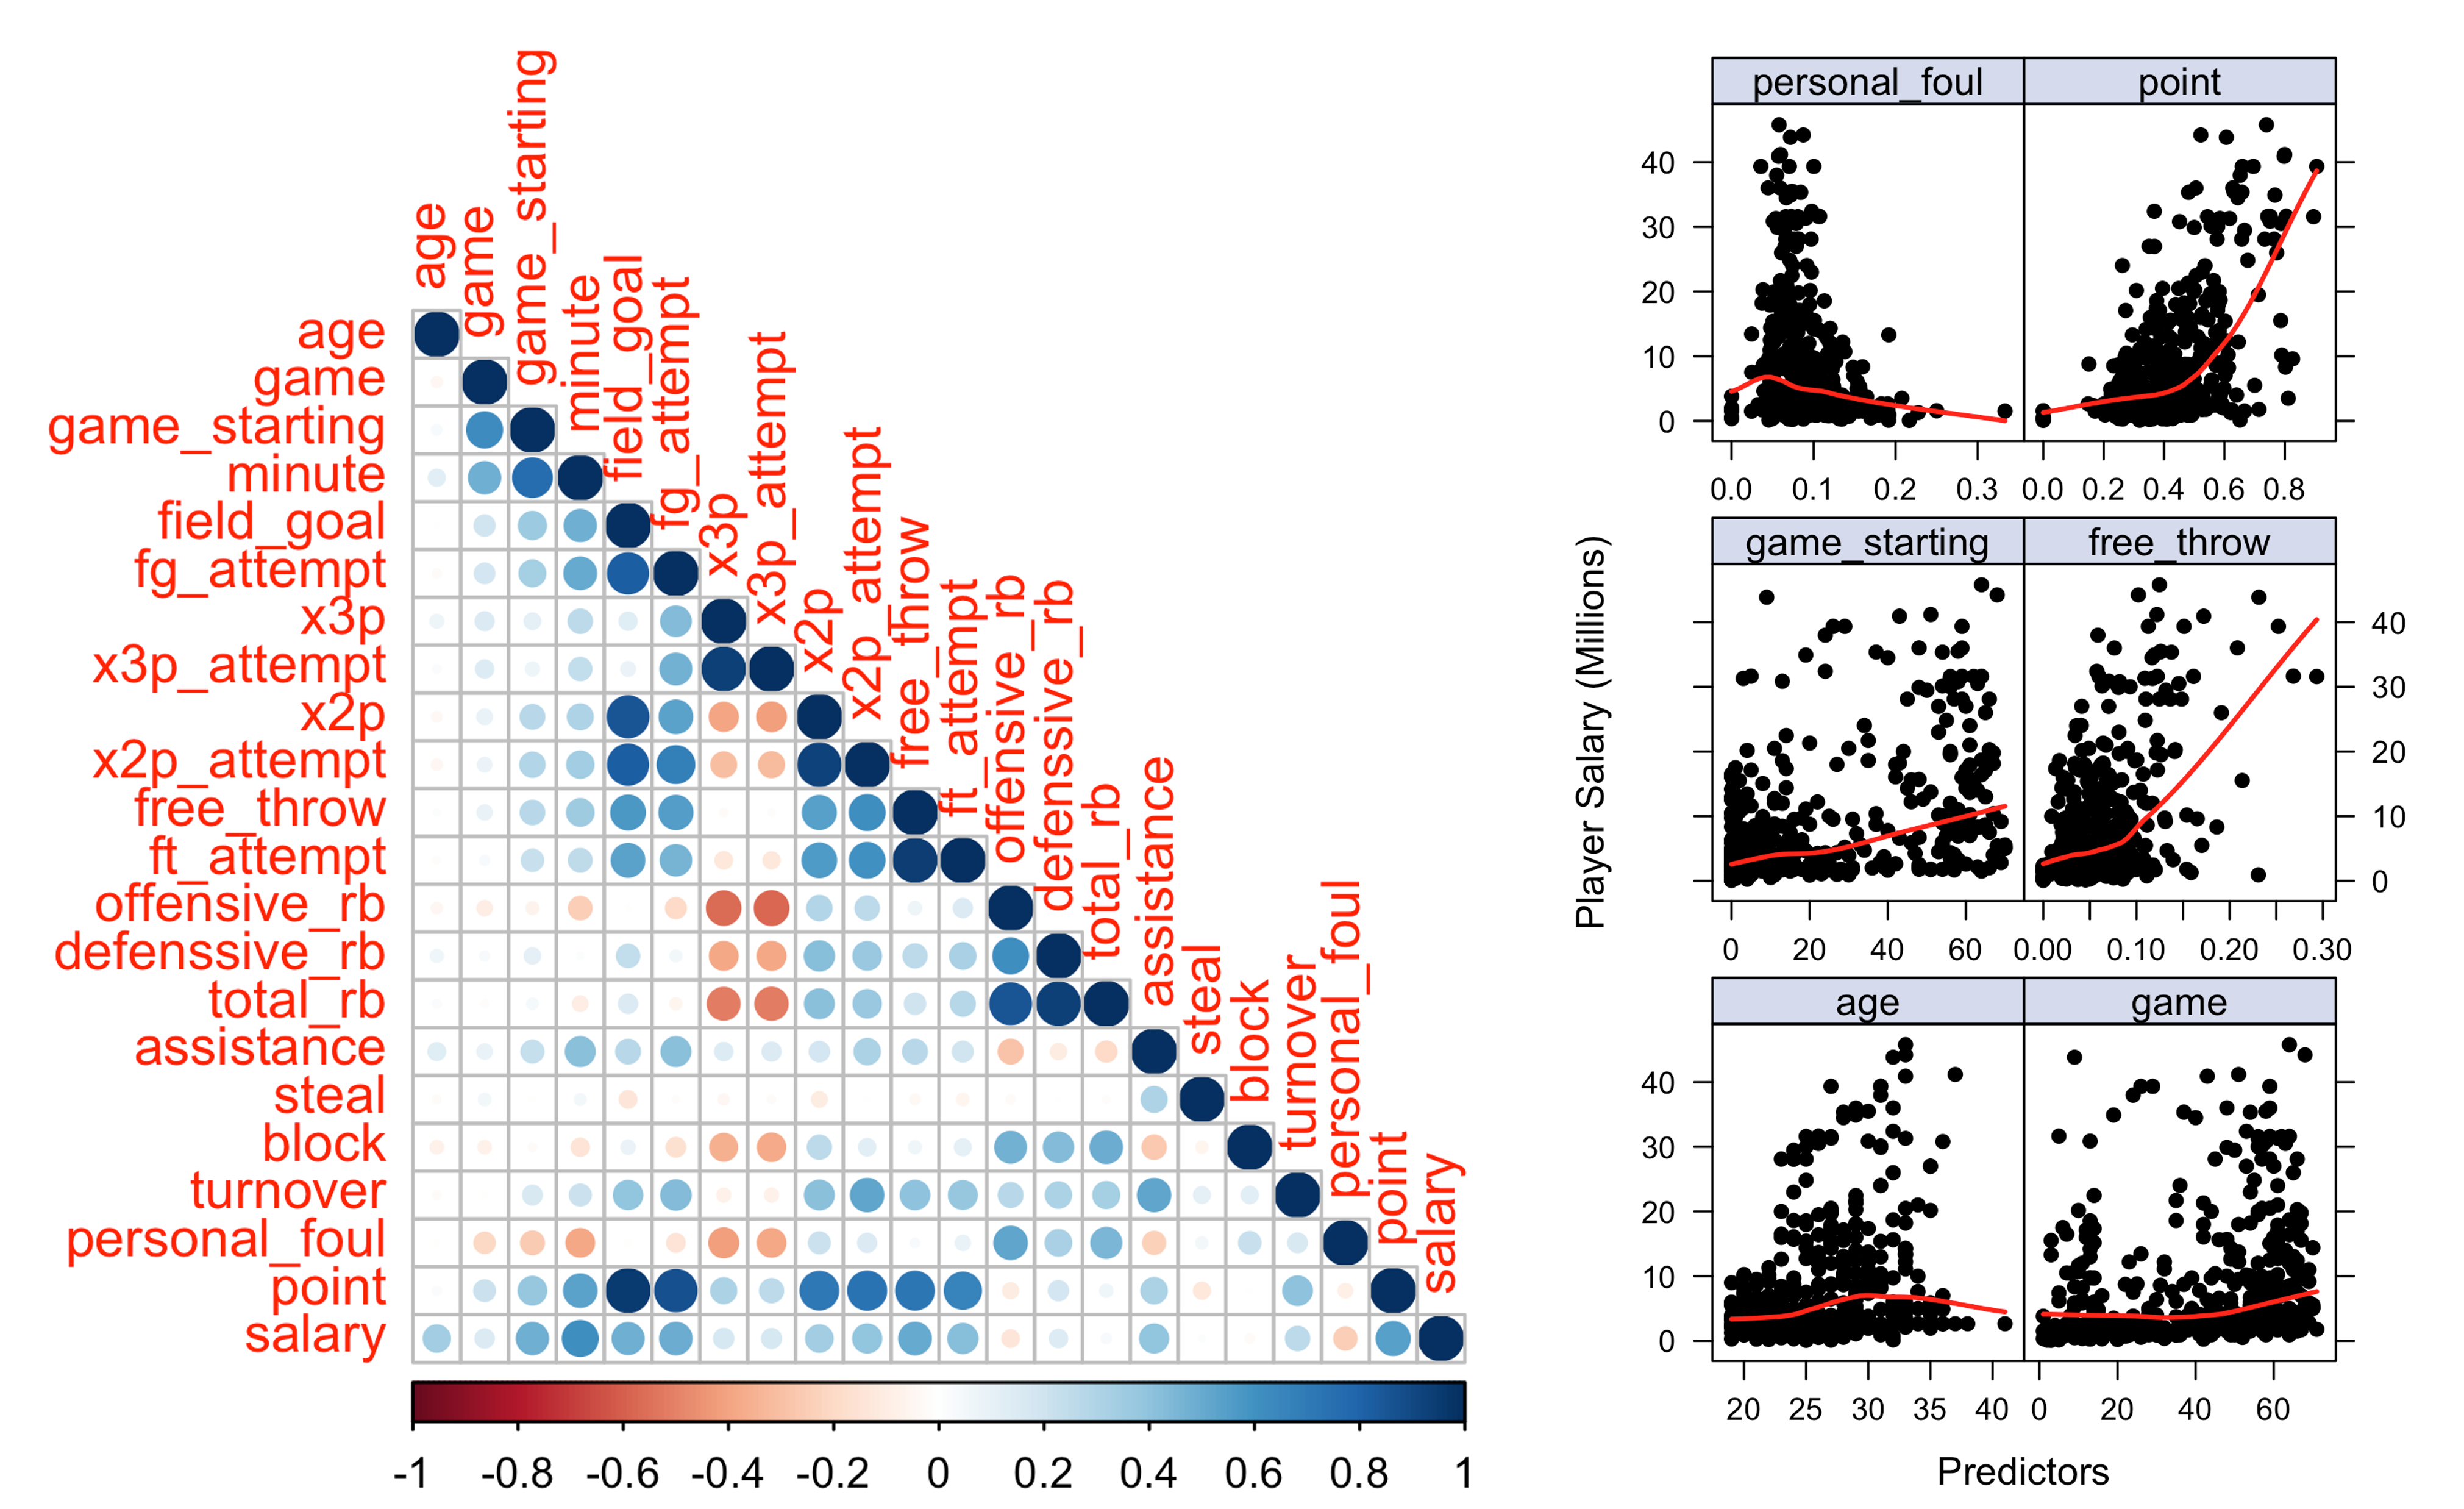
\includegraphics{report_figures/figure2_combined.png}
\caption{Correlation Heatmap and Feature Maps}
\end{figure}

\hypertarget{feature-engineering}{%
\subsection{Feature Engineering}\label{feature-engineering}}

To condense the 30-class categorical variable \texttt{team} into fewer
dummy variables, we tried clustering \texttt{team} into fewer classes
based on the median and standard deviation of player's salary in each
team. The number of clusters \(k = 3\) was chosen based on average
silhouette width (Figure 2A). The resulting clusters of \texttt{team}
were shown in Figure 2B and stored in a new
variable\texttt{team\_cluster}. Three clusters of teams are as below:

\begin{itemize}
\tightlist
\item
  Cluster 1: \texttt{BRK}, \texttt{GSW}, \texttt{LAL}, \texttt{MIA},
  \texttt{MIL}, \texttt{NOP}, \texttt{PHI}, \texttt{POR}, \texttt{UTA}
\item
  Cluster 2: \texttt{ATL}, \texttt{CHI}, \texttt{CHO}, \texttt{CLE},
  \texttt{DAL}, \texttt{DEN}, \texttt{DET}, \texttt{HOU}, \texttt{IND},
  \texttt{MEM}, \texttt{MIN}, \texttt{NYK}, \texttt{OKC}, \texttt{ORL},
  \texttt{PHO}, \texttt{SAC}, \texttt{SAS}, \texttt{TOR}
\item
  Cluster 3: \texttt{BOS}, \texttt{LAC}, \texttt{WAS}
\end{itemize}

\begin{figure}
\centering
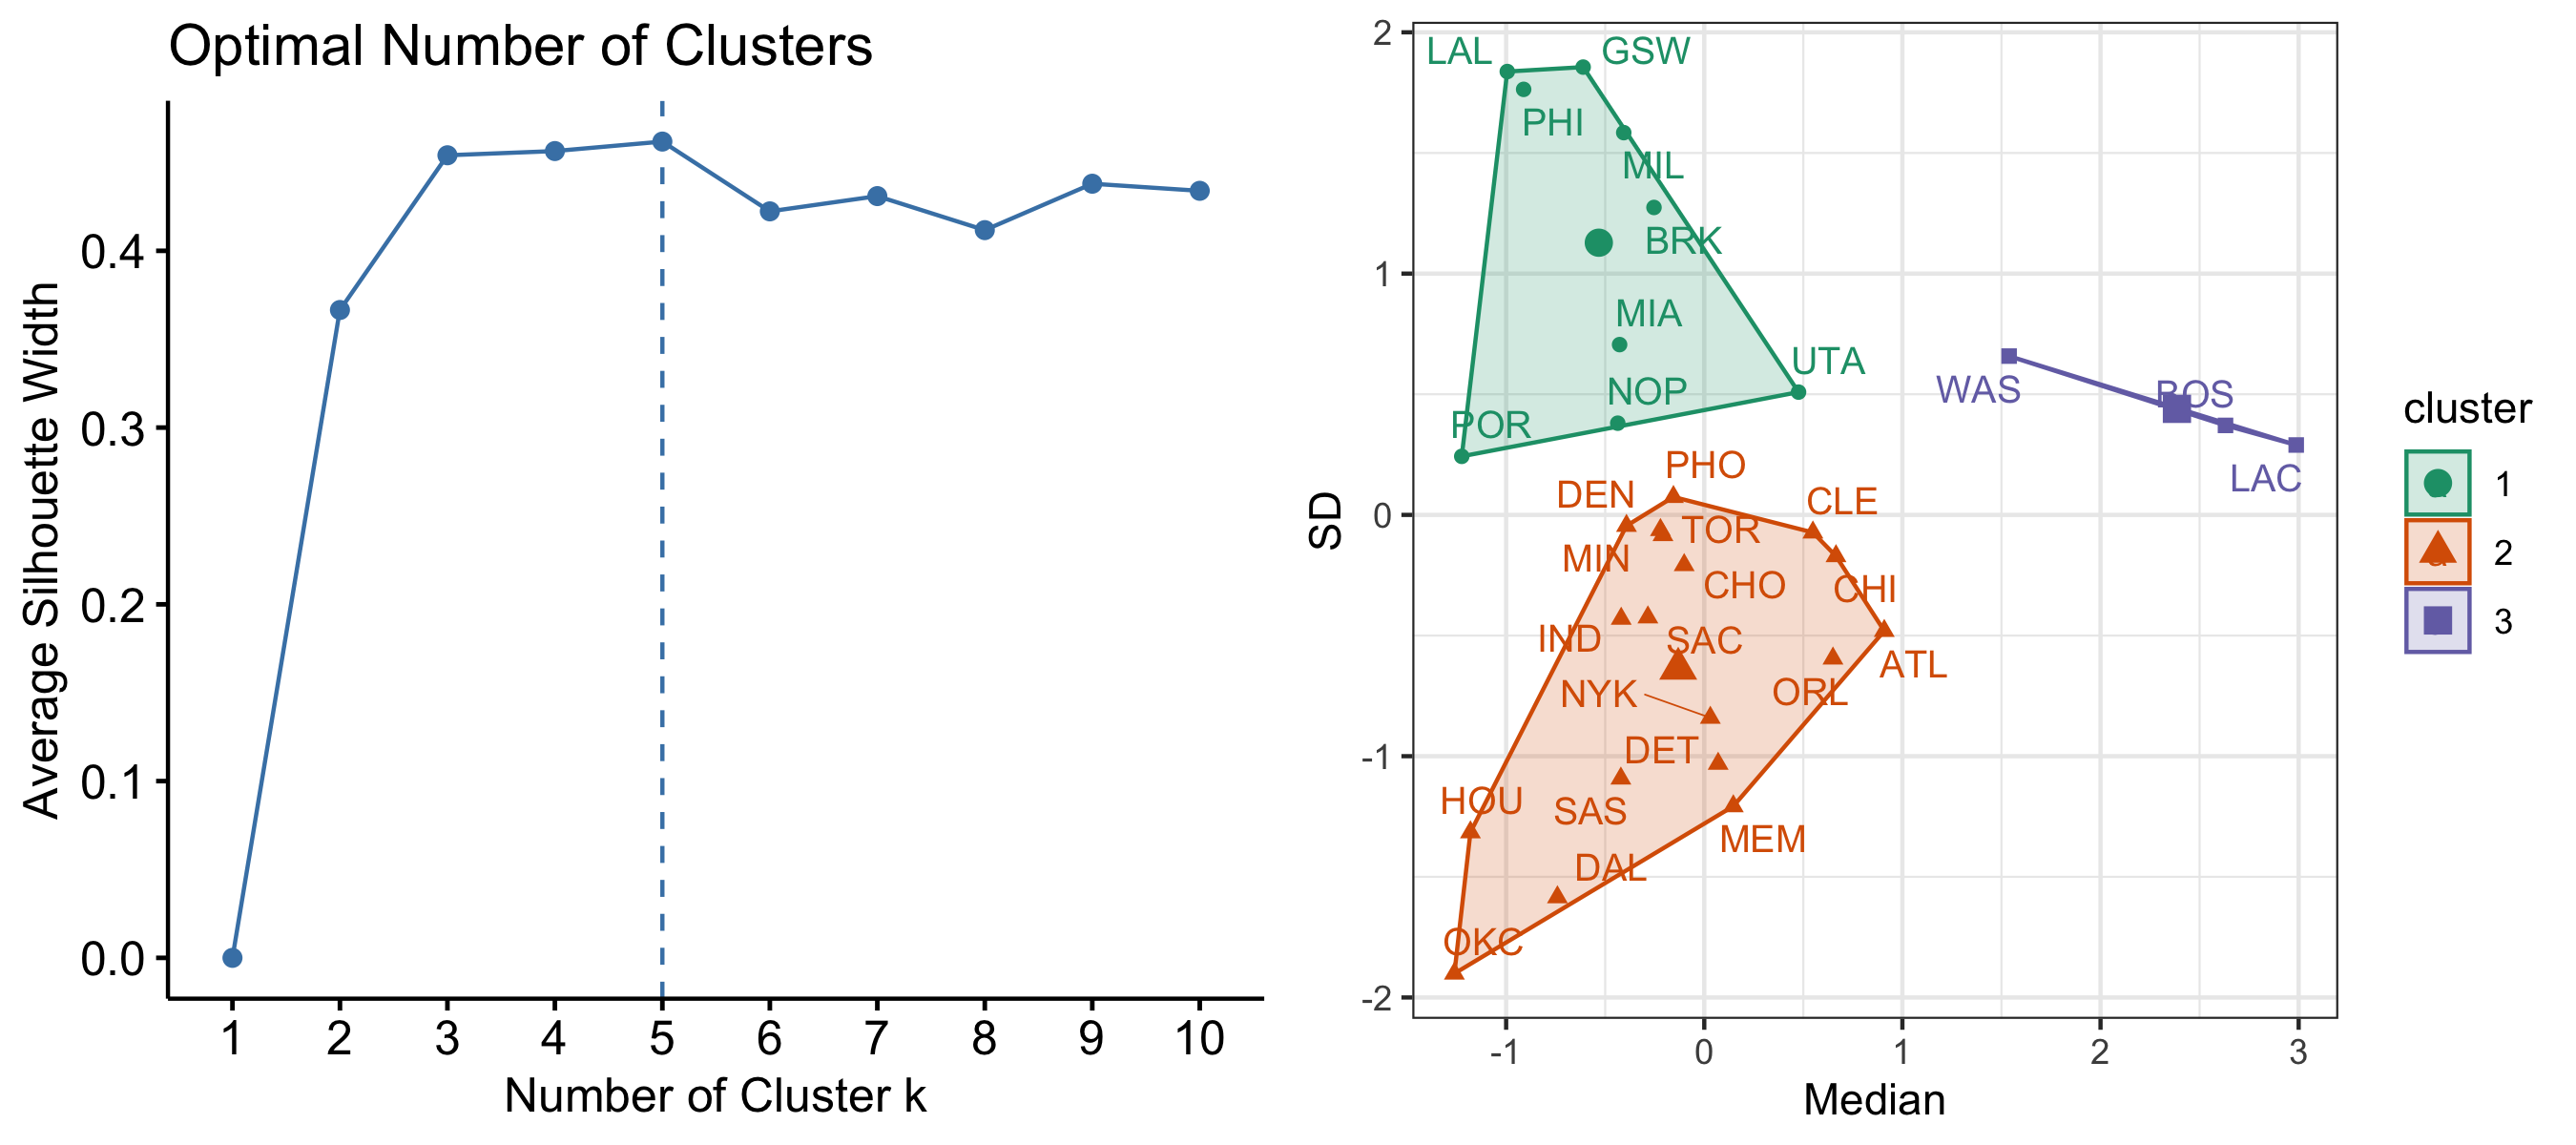
\includegraphics{report_figures/figure_tree_1.png}
\caption{Clustering on variable team}
\end{figure}

In the tree-based models, the replacement of \texttt{team} with
\texttt{team\_cluster} led to a higher prediction accuracy. For other
models, the variable \texttt{team}was still used for model construction.

\hypertarget{model-construction}{%
\subsection{Model Construction}\label{model-construction}}

After having an overview of the data, we splitted the dataset into
training (80\%) and test (20\%) set, used 10-fold repeated cross
validation to compare each model using training data, and evaluated the
model performances based on test error. We built 8 types of models in
four categories:

\begin{enumerate}
\def\labelenumi{\arabic{enumi}.}
\item
  Linear Regression Models: Standard Linear Regression Model, Elastic
  Net Model, Principal Component Regression Model (PCR)
\item
  Generalized Linear Regression: Generalized Addictive Model (GAM),
  Multivariate Adaptive Regression Splines Model (MARS)
\item
  Tree based Models Models: Random Forest (RF), Generalized Boosted
  Regression Modeling (GBM)
\item
  Neural Network
\end{enumerate}

\hypertarget{part-a---linear-regression-models}{%
\subsubsection{Part A - Linear Regression
Models}\label{part-a---linear-regression-models}}

\hypertarget{standard-least-squared}{%
\paragraph{(1) Standard Least-Squared}\label{standard-least-squared}}

Standard Least-Squared model is used for a reference of other models, as
it may not perform well given the presence of multicolinearity and
nonliner trend in the data. There is no tuning parameter for standard
least-squared model.

\hypertarget{elastic-net}{%
\paragraph{(2) Elastic Net}\label{elastic-net}}

The elastic-net model has two parameters, which are \(\alpha\)
(compromise between LASSO and ridge) and \(\lambda\) (the penalty term
limits the number or magnitude of predictor coefficients). The
elastic-net model reached its best tune at \(\alpha = 0.6\) and
\(\lambda = 0.44\) (see Appendix B Figure1).

\hypertarget{principle-component-regression}{%
\paragraph{(3) Principle Component
Regression}\label{principle-component-regression}}

The tuning parameter of PCR is the number of principal components (PCs)
included in the final model. There are 12 PCs included in the model with
minimum RMSE (see Appendix B).

\hypertarget{part-b---generalized-linear-regression-models}{%
\subsubsection{Part B - Generalized Linear Regression
Models}\label{part-b---generalized-linear-regression-models}}

\hypertarget{gam}{%
\paragraph{(4) GAM}\label{gam}}

There is no tuning parameter for GAM. The GAM model can capture the
non-linear trend in the model, but it may have a high variance.
\texttt{age}, \texttt{game\_starting}, \texttt{assistance},
\texttt{personal\_foul}, and \texttt{point} are statistically
significant predictors at 0.0001 significant level.

\hypertarget{mars}{%
\paragraph{(5) MARS}\label{mars}}

The tuning parameter for MARS is \texttt{nprune} and \texttt{degree}.
When attempting to fit the MARS model, we noticed that the RMSE
increased drastically when degree is over 3 and nprune is over 8.
Therefore, we would choose the range of degrees as 1:4 and range of
nprune as 2:8. When \texttt{nprune\ =\ 6} and \texttt{degree\ =\ 3},
MARS model reached its best tune and RMSE is lowest. 6 of 54 predictors
are included in the mdoel, and the top 3 important predictors are:
\texttt{age}, \texttt{minute}, \texttt{game}. MARS model is highly
adaptive comparing with previous models and has a higher prediction
accuracy (see Appendix B).

\hypertarget{part-c-tree-based-models}{%
\subsubsection{Part C: Tree-Based
Models}\label{part-c-tree-based-models}}

\hypertarget{random-forest}{%
\paragraph{(6) Random Forest}\label{random-forest}}

Tuning parameter for random forest regression in package \texttt{ranger}
are \texttt{mtry} (number of variables to split at in each node) and
\texttt{min.node.size} (minimal size of each node). Through 10-fold
repeated CV (see Appendix C), the optimal random forest model have
parameters \texttt{mtry\ =\ 26} and \texttt{min.node.size\ =\ 1}. Random
forest preserve the advantage of single decision trees that can handle
correlation between variables and non-linearity. However, since here
\texttt{mtry\ =\ 26} equals our total number of variables, this random
forest estimator may not well decorrelate single trees, and thus may
overfit the dataset.

\hypertarget{generalized-boosted-regression-modeling-gbm}{%
\paragraph{(7) Generalized Boosted Regression Modeling
(GBM)}\label{generalized-boosted-regression-modeling-gbm}}

Tuning parameters for Generalized boosted regression modeling (GBM) are
\texttt{n.trees} (total number of trees to fit),
\texttt{interaction.depth} (maximum depth of each tree),
\texttt{shrinkage} (learning rate), and \texttt{n.minobsinnode} (minimum
number of observations in the terminal nodes). Through 10-fold repeated
CV (see Appendix C), the optimal random forest model have parameters
\texttt{n.trees\ =\ 6000}, \texttt{interaction.depth\ =\ 5},
\texttt{shrinkage\ =\ 0.0008}, and \texttt{n.minobsinnode\ =\ 1}.

\hypertarget{part-d-neural-network}{%
\subsubsection{Part D: Neural Network}\label{part-d-neural-network}}

Several 2-hidden layer neural networks were built to fit the data. The
optimal model fitted after parameter tuning is a 2-hidden layer neural
network with \(n_1 = 10\) and \(n_2 = 5\) nodes in the first and second
layers, applying dropout regularization. Figure 3B shows the resulting
MSE in the training and validation sets after 250 epochs.

As shown in Figure 3C, as the number of nodes in the first and second
hidden layers increases, neural networks can provide very accurate
fittings of the training data, with much lower MSEs compared to other
methods. However, the predictions are not satisfying when the models are
applying to the test data.

Despite trying different number of nodes and applying regularization
techniques (L2 and dropout), the resulting models still have a
noticeable overfitting problem. Given the size of the dataset is very
small (\(n=442\)), the performance of neural network is not as good as
some traditional statistical models. It is more useful when the size of
dataset is much larger with more variables.

\begin{figure}
\centering
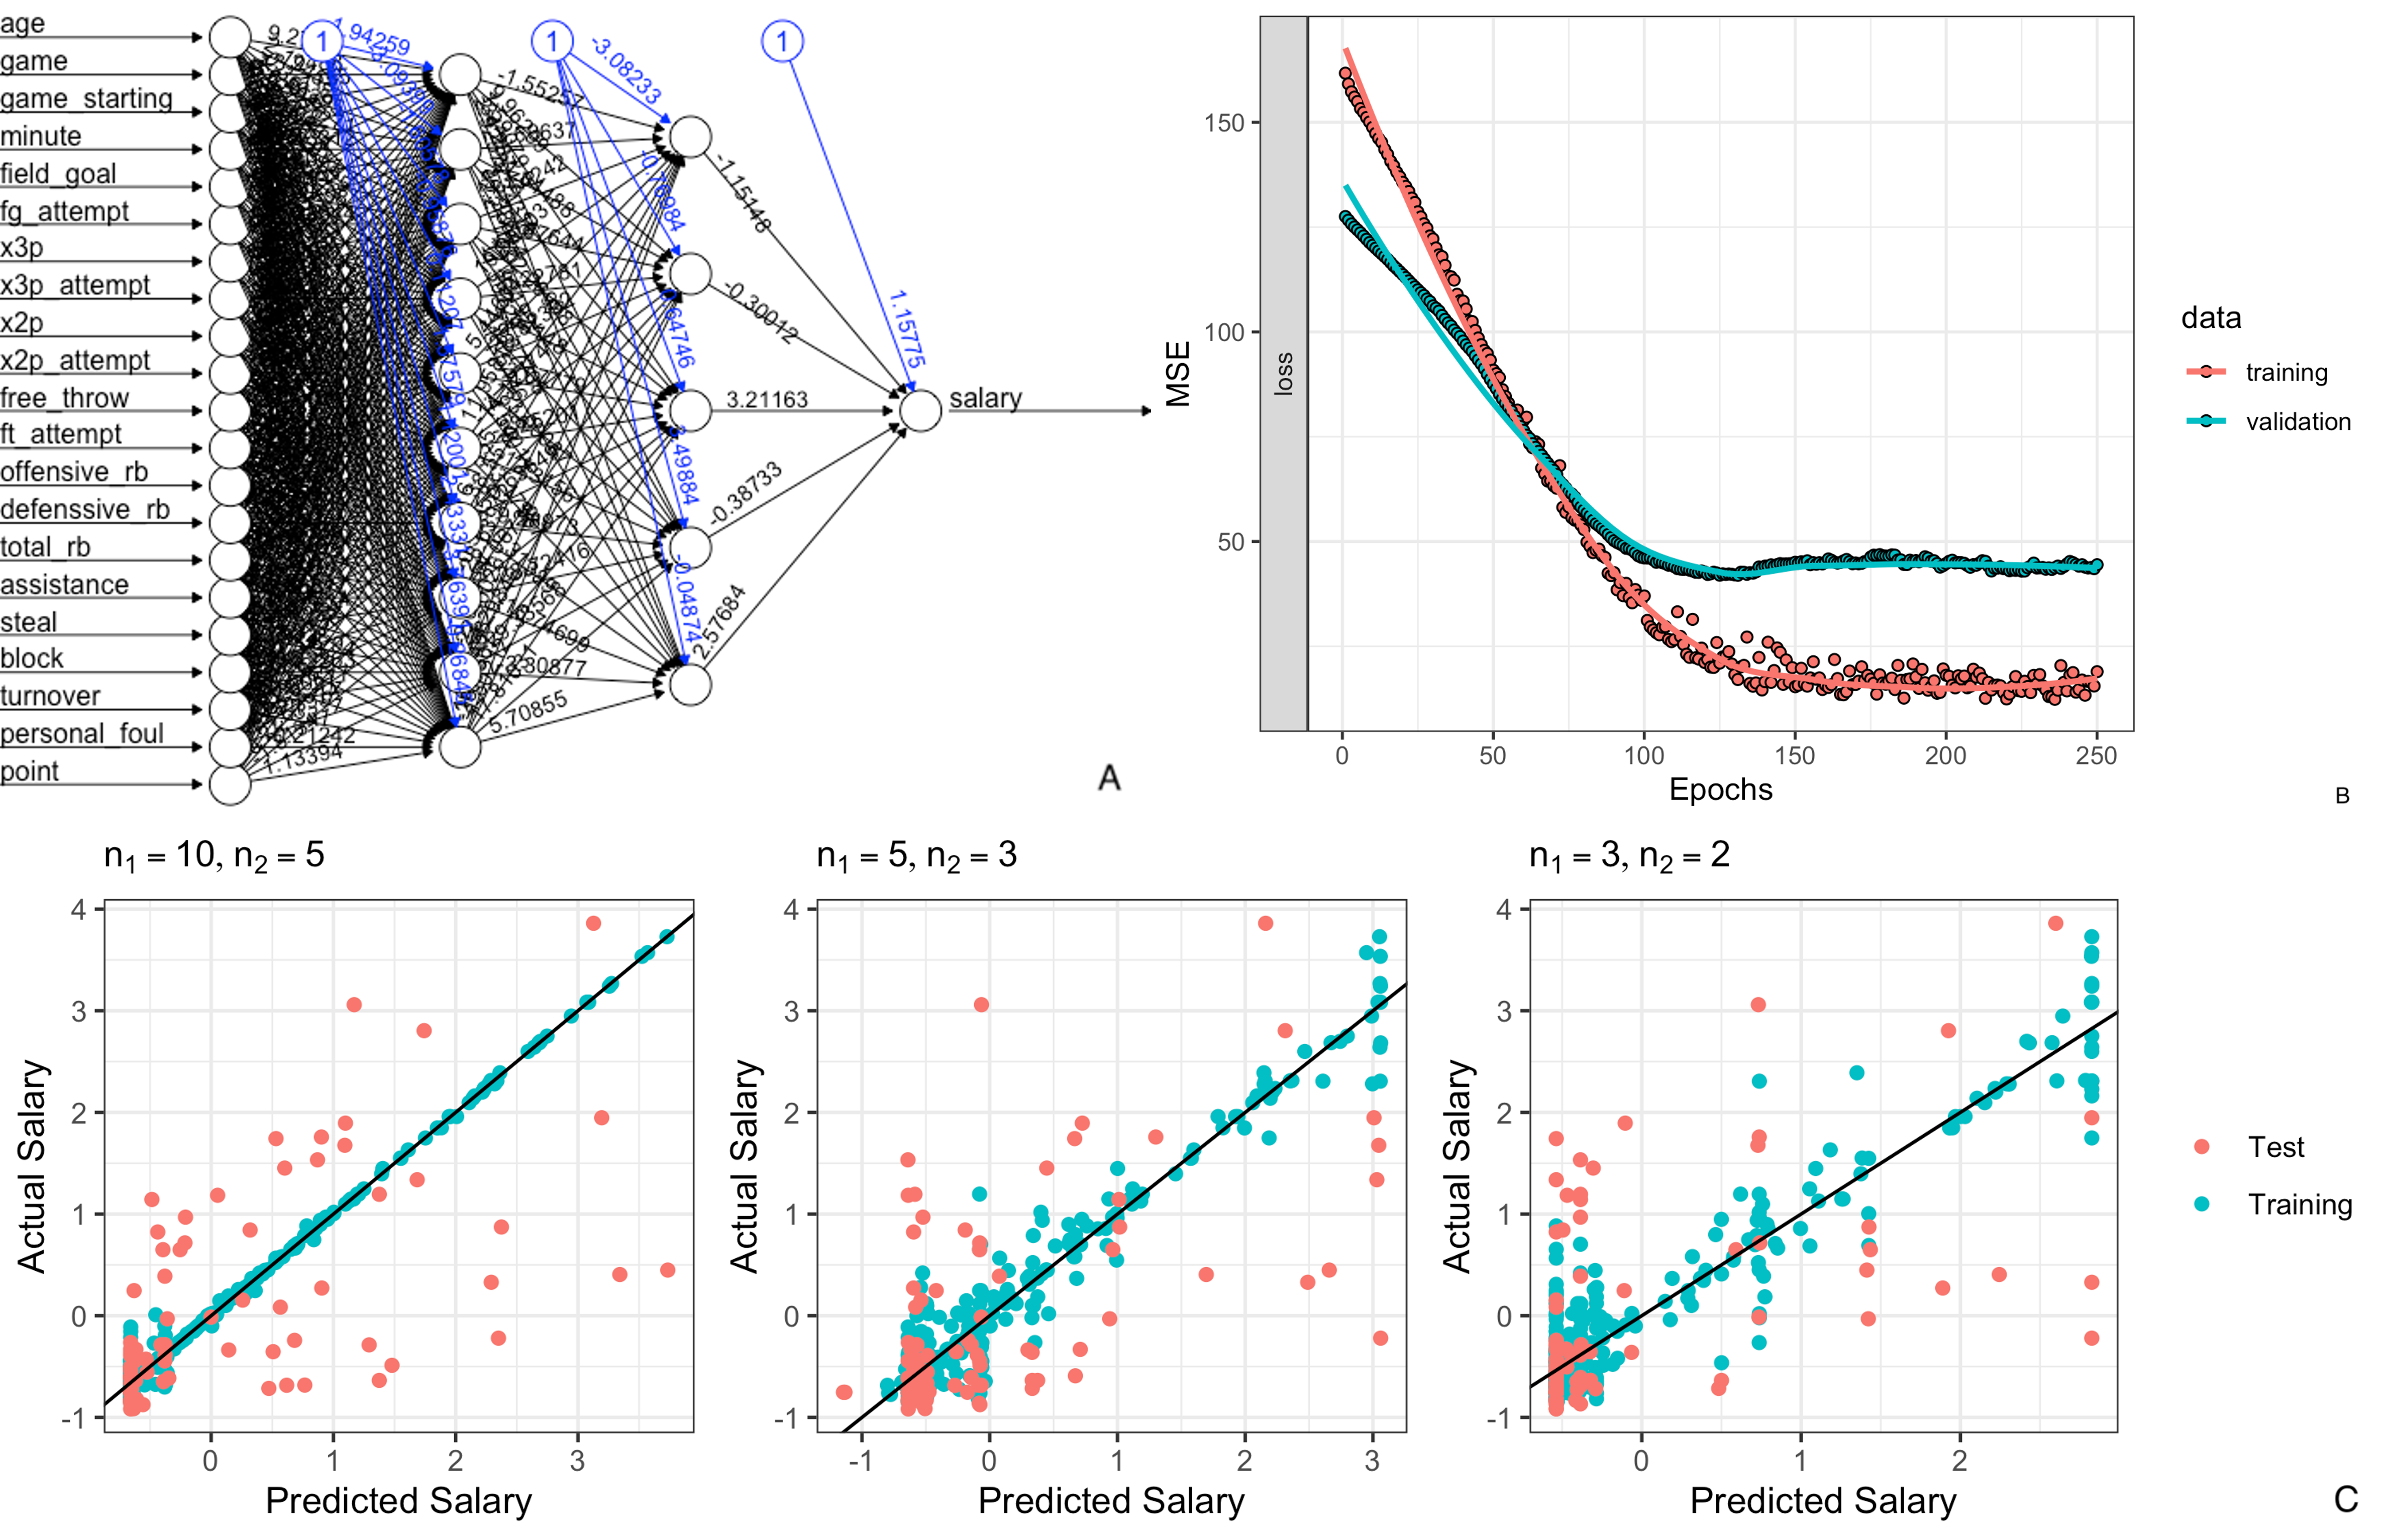
\includegraphics{report_figures/figure_nn.png}
\caption{Structure and MSE of the resulting 2-hidden layer neural
network}
\end{figure}

\hypertarget{model-comparasion-and-final-model-interpretation}{%
\subsection{Model Comparasion and Final Model
Interpretation}\label{model-comparasion-and-final-model-interpretation}}

\hypertarget{model-comparison}{%
\subsubsection{Model Comparison}\label{model-comparison}}

The 10-fold CV RMSE (validation set RMSE for neural network) and test
set RMSE for all candidate models are shown in Table 2. The GBM model
has the best performance in terms of both CV and test errors.

\begin{longtable}[]{@{}lllllllll@{}}
\caption{Summary of Model Performance}\tabularnewline
\toprule
& Linear & ElasticNet & PCR & GAM & MARS & RandomForest & GBM &
NeuralNetwork \\
\midrule
\endfirsthead
\toprule
& Linear & ElasticNet & PCR & GAM & MARS & RandomForest & GBM &
NeuralNetwork \\
\midrule
\endhead
Training RMSE & 6.79 & 6.45 & 7.16 & 6.84 & 6.06 & 5.42 & 5.41 & 6.40 \\
Test RMSE & 6.66 & 6.04 & 5.39 & 6.84 & 5.16 & 4.83 & 4.75 & 6.64 \\
\bottomrule
\end{longtable}

\hypertarget{final-model-interpretation}{%
\subsubsection{Final Model
Interpretation}\label{final-model-interpretation}}

Based on the CV RMSE and validation set RMSE, our best model is the
Generalized Boosted Regression Modeling (GBM) with tuning parameters:

\begin{itemize}
\item
  \texttt{n.trees\ =\ 6000}
\item
  \texttt{interaction.depth\ =\ 5}
\item
  \texttt{shrinkage\ =\ 0.0008}:
\item
  \texttt{n.minobsinnode\ =\ 1}
\end{itemize}

10 most important variables (computed from permuting OOB data) are
\texttt{minute}, \texttt{age}, \texttt{point}, \texttt{free\_throw},
\texttt{fg\_attempt}, \texttt{game\_starting}, \texttt{assistance},
\texttt{ft\_attempt}, \texttt{team\_cluster}, and \texttt{defensive\_rb}
(Figure 4).

\begin{figure}
\centering
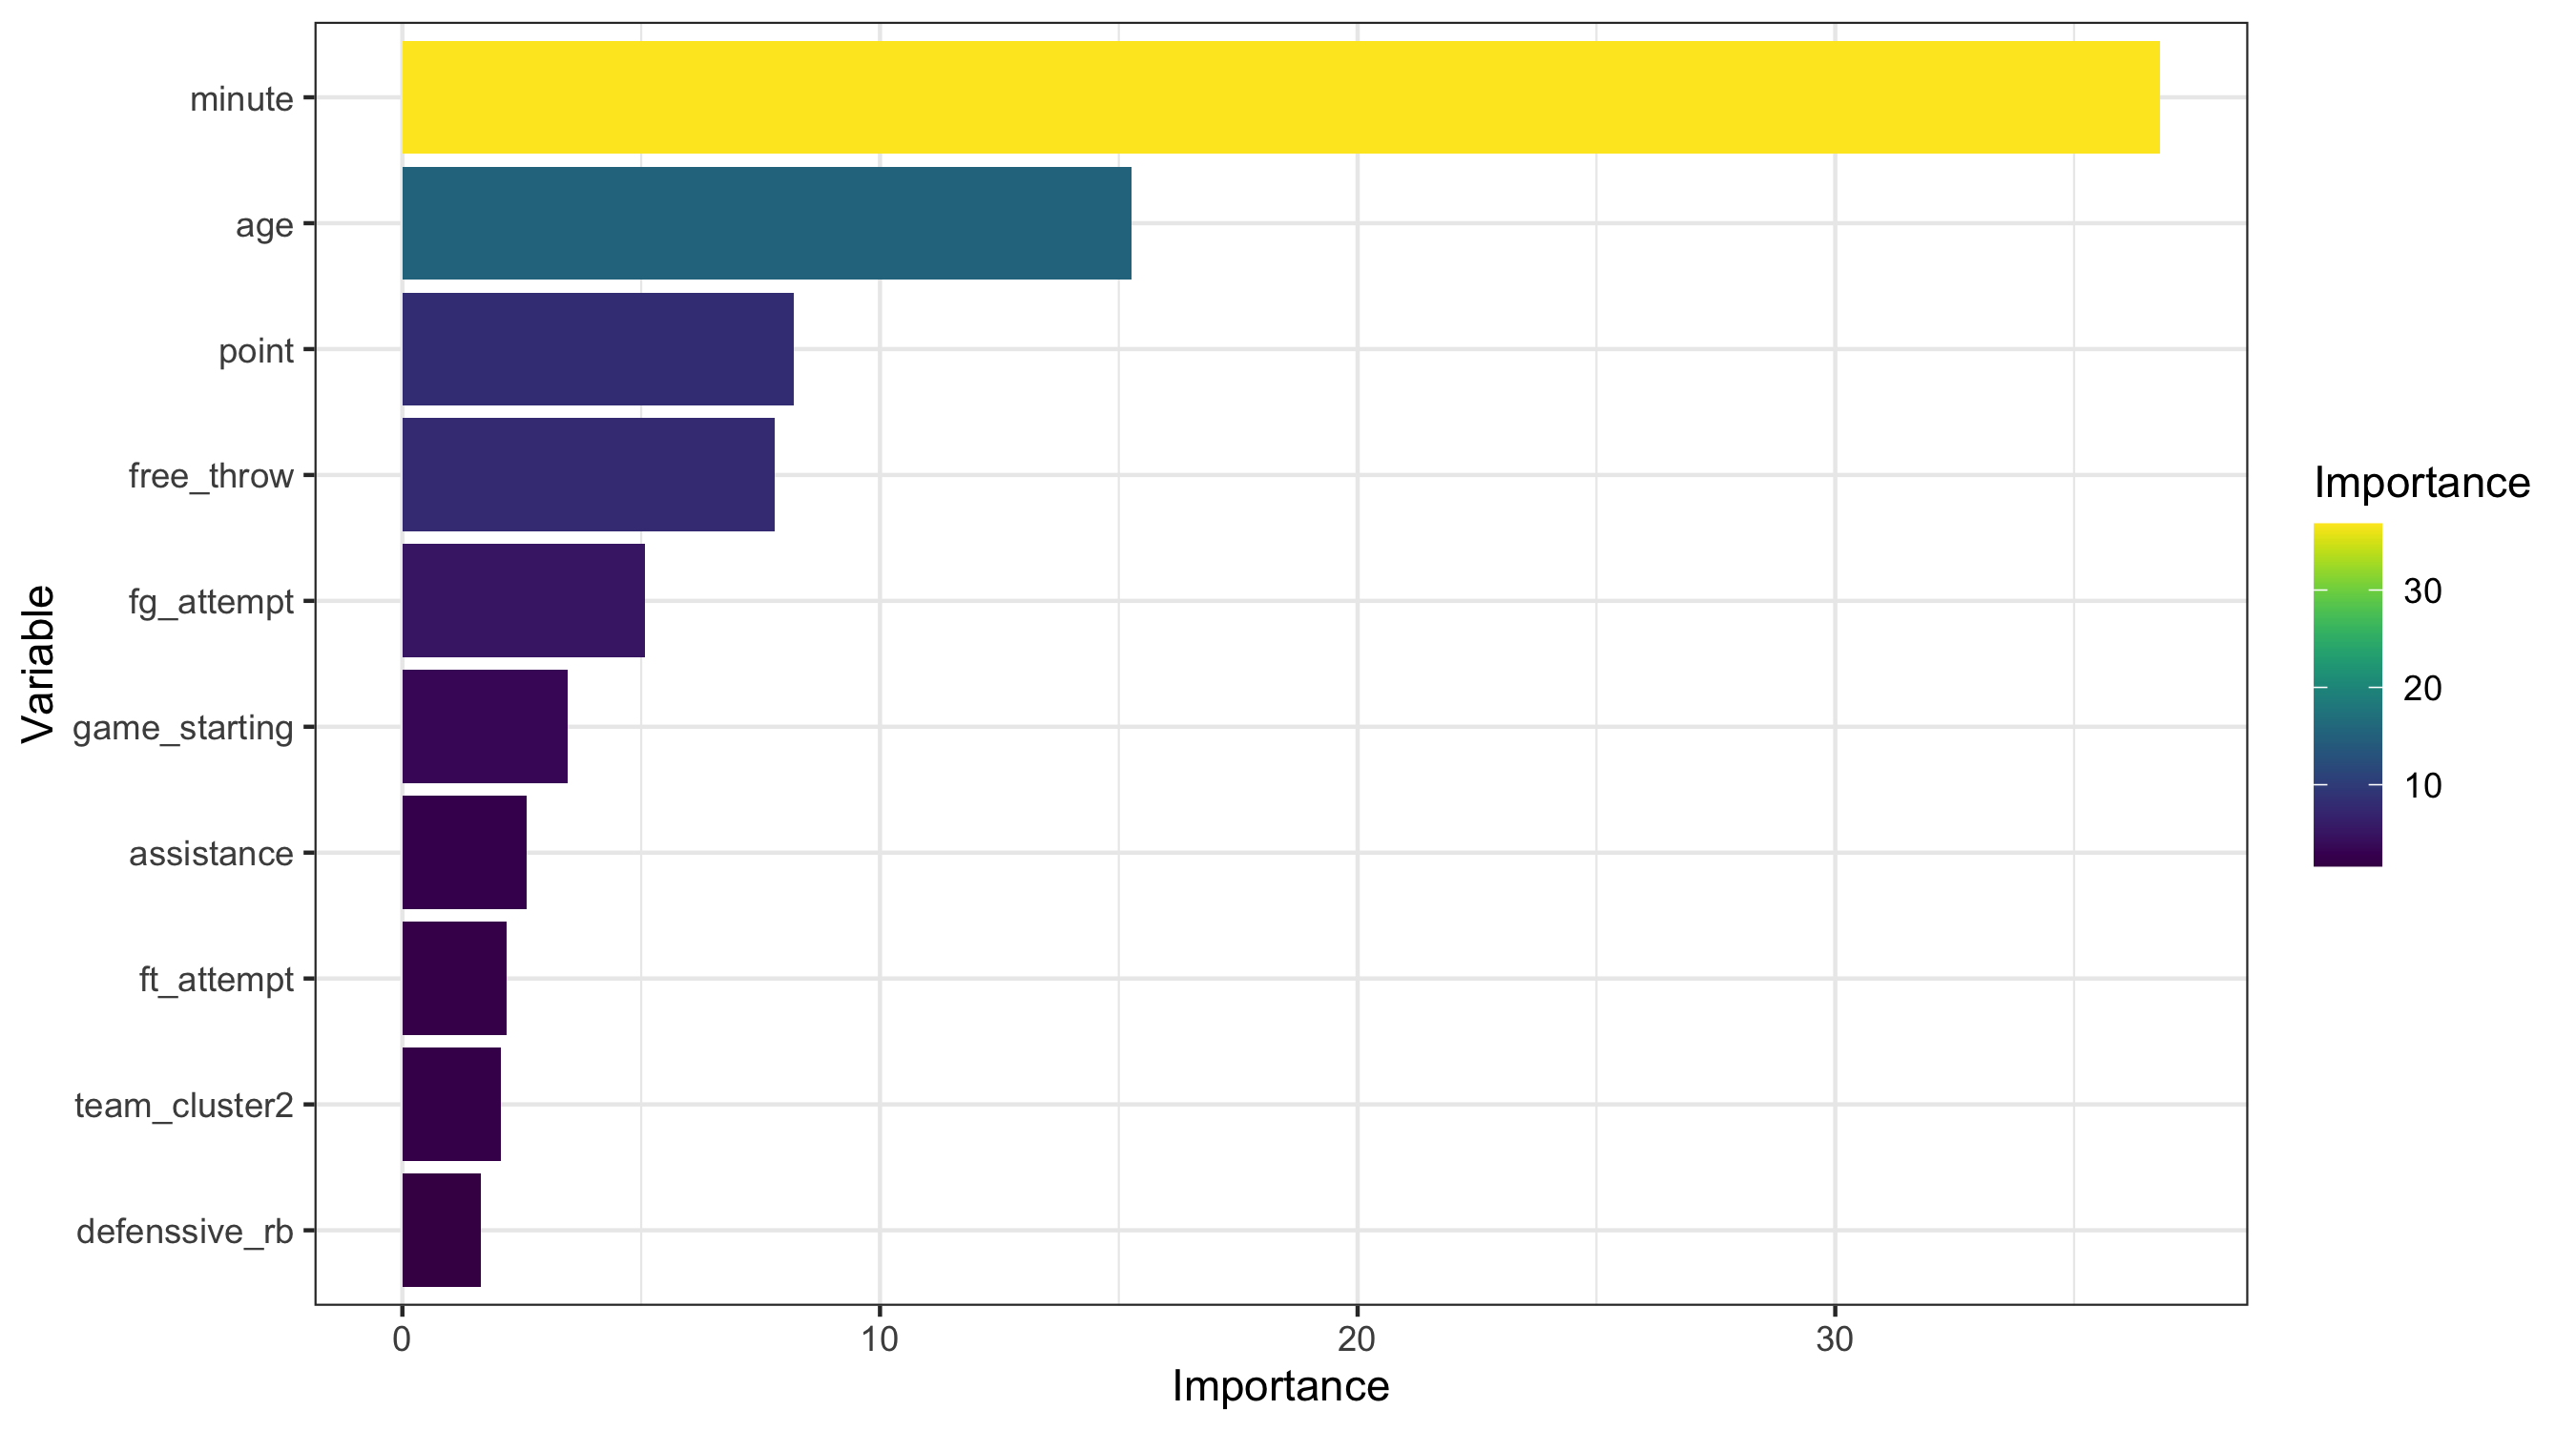
\includegraphics{report_figures/figure_tree_3.png}
\caption{Variable Importance of GBM model}
\end{figure}

With our fitted GBM model, we can make prediction on new observations.
The RMSE on our test data is 4.745948.

Given that GBM is a black-box model, we refer to \texttt{lime} package
to achieve explanations of the result of the model on new observations,
by fitting a simpler model to the permuted data with the above 15 most
important features. Table 3 displays 6 randomly selected observations
from the test data. The players' name, true salary (in million), and
predicted salary from GBM are shown.

\begin{longtable}[]{@{}lrr@{}}
\caption{Prediction on Randomly Selected New
Observations}\tabularnewline
\toprule
player & salary (true) & salary (predicted by GBM) \\
\midrule
\endfirsthead
\toprule
player & salary (true) & salary (predicted by GBM) \\
\midrule
\endhead
Cade Cunningham & 10.050120 & 8.590867 \\
Cam Reddish & 4.670160 & 3.627087 \\
Christian Wood & 13.666667 & 14.730414 \\
Corey Kispert & 3.383640 & 3.248053 \\
D'Angelo Russell & 30.013500 & 14.735256 \\
Danuel House Jr. & 2.045094 & 4.792719 \\
\bottomrule
\end{longtable}

The explanation of the GBM model from lime are shown in Figure 5. Inside
the plot, the x-axis shows the relative strength of each variables, and
positive values (blue) show that the the variable increase the value of
the prediction, while the negative values (red) decrease the prediction
value.

\begin{figure}
\centering
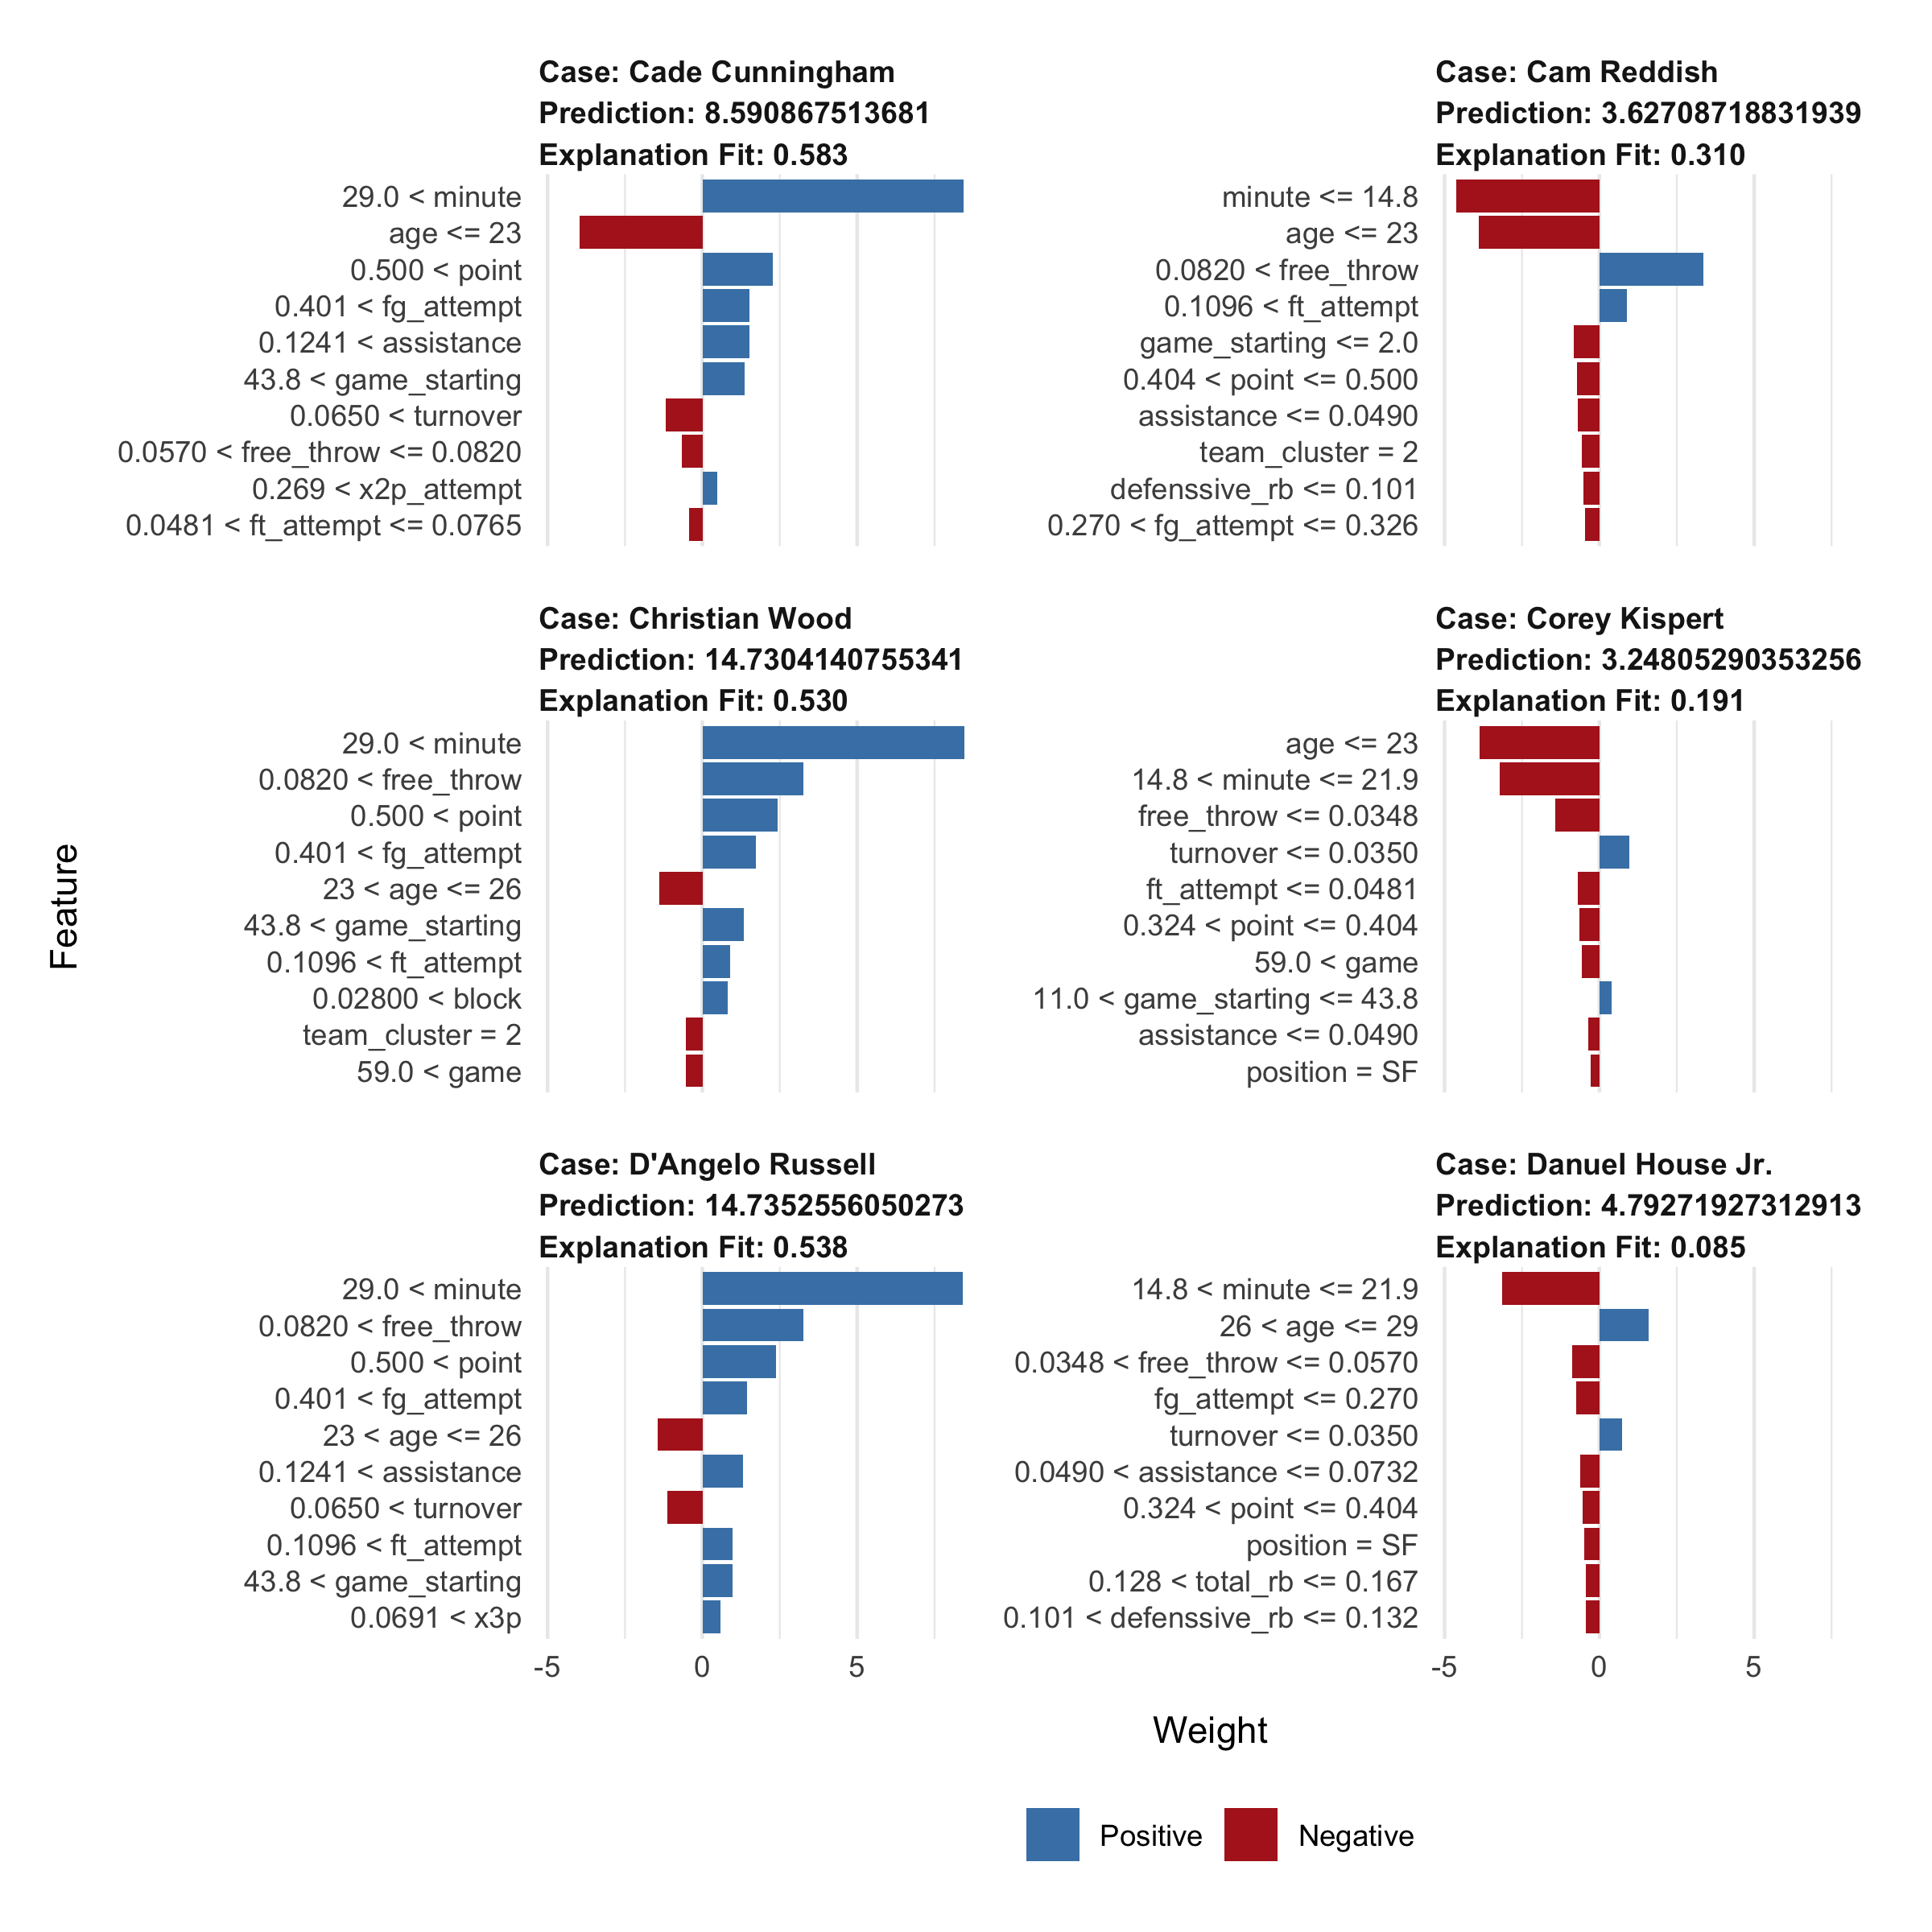
\includegraphics[width=\textwidth,height=0.5\textheight]{report_figures/figure_tree_4.png}
\caption{Explanation of final GBM model from lime package}
\end{figure}

Take the first case of player Cade Cunningham as an example. Cade's true
salary is 10.050120 million. His predicted salary from GBM is 8.590868
million, which are quite similar to each other. Among the 10 most
important variables, factors \texttt{mintue\ \textgreater{}\ 90},
\texttt{point\ \textgreater{}\ 0.5},
\texttt{game\_starting\ \textgreater{}\ 43.8},
\texttt{assistance\ \textgreater{}\ 0.1241},
\texttt{fg\_attempt\ \textgreater{}\ 0.401} and
\texttt{x2p\_attempt\ \textgreater{}\ 0.269} increases Cade's salary,
while factors \texttt{age\ \textless{}=\ 23},
\texttt{turnover\ \textgreater{}\ 0.065},
\texttt{0.057\ \textless{}\ free\_throw\ \textless{}=\ 0.082} and
\texttt{team\_cluster\ =\ 2} decreases his salary.

\hypertarget{conclusion}{%
\subsection{Conclusion}\label{conclusion}}

In this project, we explored different ways of building statistical
models to predict the salary of NBA players based on their game
statistics. We preprocessed the original raw data by removing missing
values, joining datasets, and deriving more meaningful variables based
on the existing ones. We then conducted an exploratory analysis to
detect useful patterns in variable distribution and their correlations.
To deal with the problems emerging from the preliminary analysis, such
as co-linearity, non-linearity, and a large number of dummy variables,
we did feature engineering to collapse categories, conducted variable
selection to reduce model dimensions, applied various regularization
techniques to prevent model overfitting, and introduced more
sophisticated statistical methods to capture non-linear relationships.
Among the 8 models fitted, we selected the GBM as the final predictive
model after evaluating their performances on cross validation RMSE.
Applying the final model on the test set, it also achieved a small RMSE
value, indicating an excellent prediction accuracy and a low level of
over-fitting. Other models did not achieve the same level of prediction
accuracy as the GBM, either underfitting the data with higher RMSE on
the training set or fitting the training data too well (particularly, in
the case of the neural network model).

From the GBM model, we also gained insights into important variables
that influence the player's salary, among which the top 10 variables are
\texttt{minute}, \texttt{age}, \texttt{point}, \texttt{free\_throw},
\texttt{fg\_attempt}, \texttt{game\_starting}, \texttt{assistance},
\texttt{ft\_attempt}, \texttt{team\_cluster}, and
\texttt{defensive\_rb}. These findings are consistent with our
understanding of factors that commonly affect the income of NBA players.

The study has several limitations. Interaction analysis can be conducted
in the family of linear regression models. In building the neural
network, we only used trained the multilayer perceptron with the ReLU
activation functions. Several other model structures and activation
functions are worth trying in the future. The model accuracy can be
further improved by introducing new variables. For example, the current
salary level of a player should be more related to his performance in
the year before making the new contract. Therefore, apart from the
statistics for 2021-2022 season, player data from previous seasons can
also be included in the analysis. Furthermore, some players having a
high salary may suffer injuries in recent games; injury data can also be
taken into account.

\newpage

\hypertarget{references}{%
\subsection{References}\label{references}}

{[}1{]}\url{https://www.basketball-reference.com/contracts/players.html}

{[}2{]}\url{https://www.basketball-reference.com/leagues/NBA_2022_per_game.html}

{[}3{]}\url{https://www.geeksforgeeks.org/how-neural-networks-are-used-for-regression-in-r-programming/}

\newpage

\hypertarget{appendices}{%
\subsection{Appendices}\label{appendices}}

\hypertarget{appendix-a---numeric-variable-distribution}{%
\subsubsection{Appendix A - Numeric Variable
Distribution}\label{appendix-a---numeric-variable-distribution}}

\begin{figure}
\centering
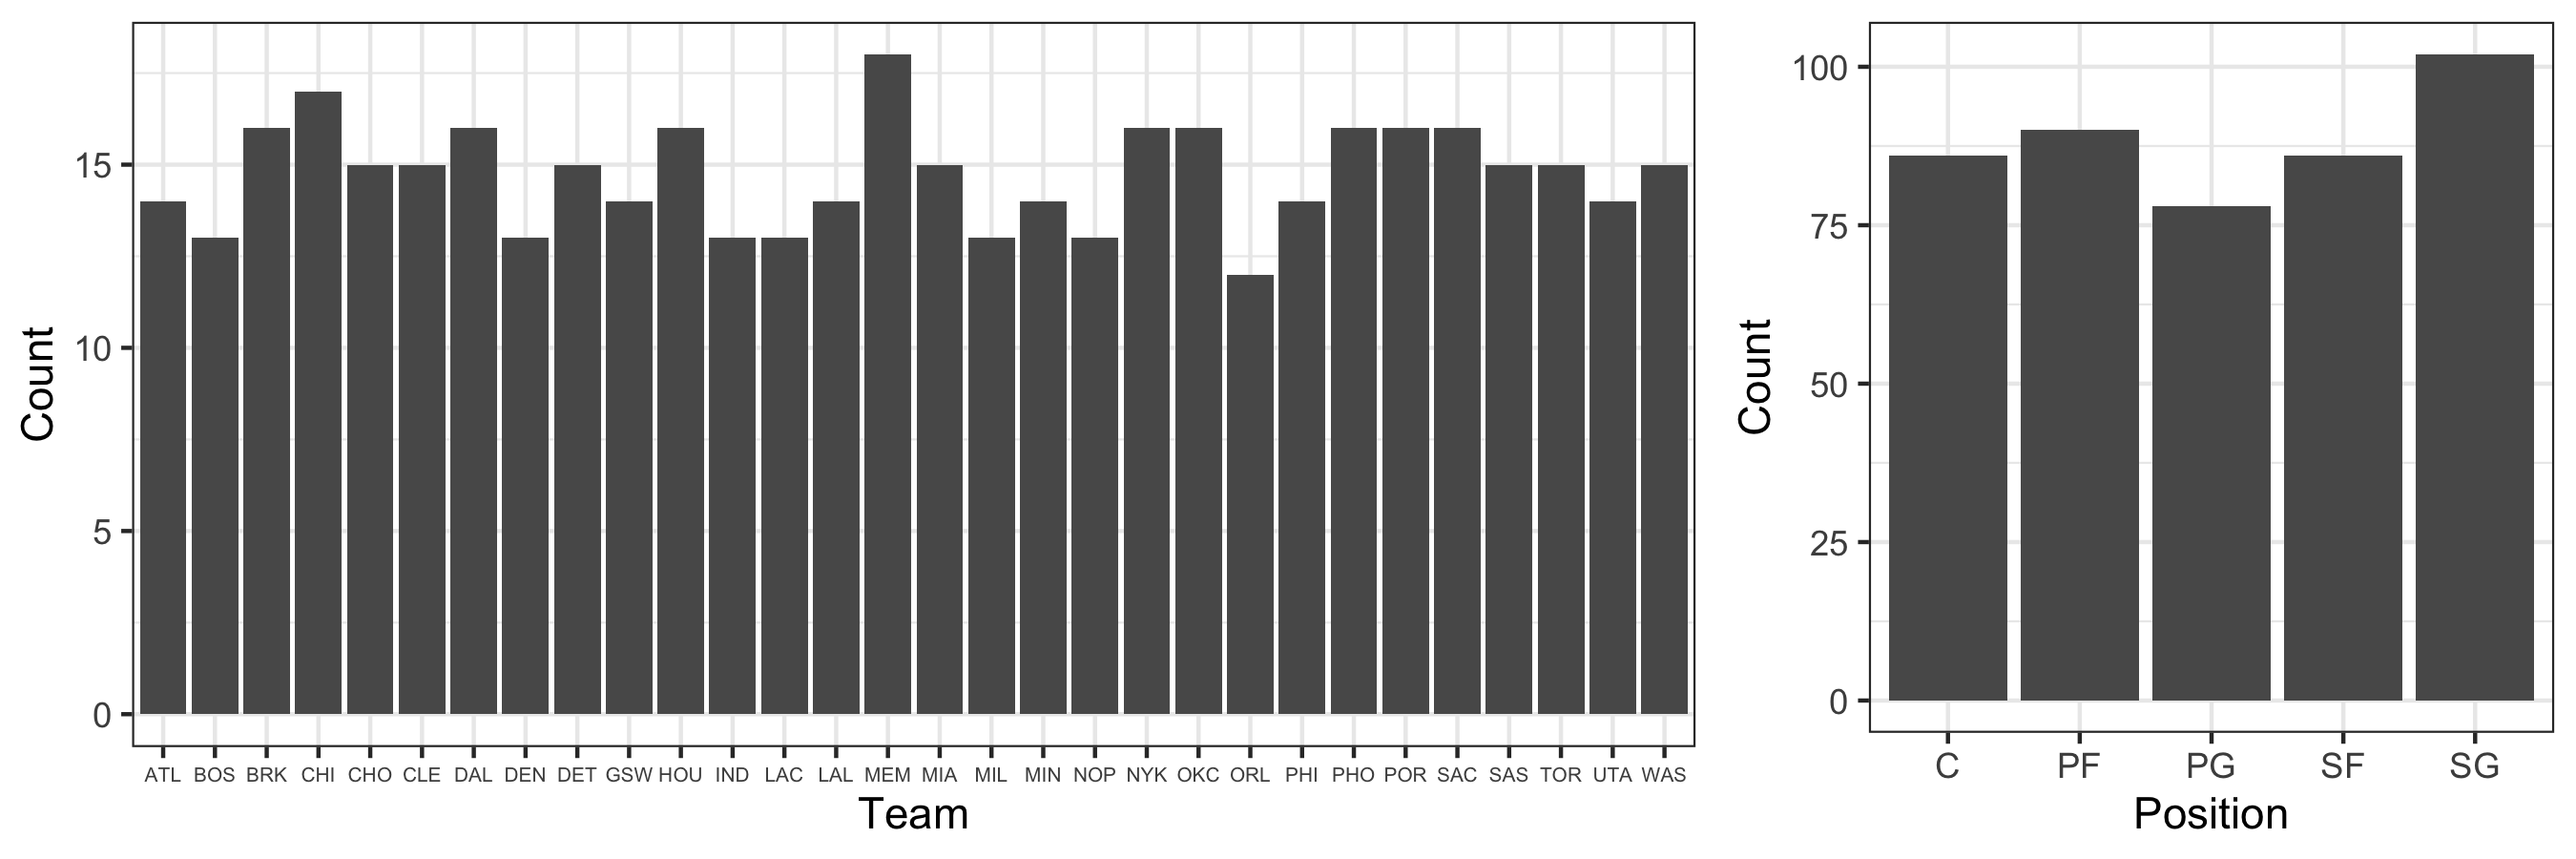
\includegraphics{report_figures/figure_1.png}
\caption{Histograms of Predictive Variables}
\end{figure}

\begin{figure}
\centering
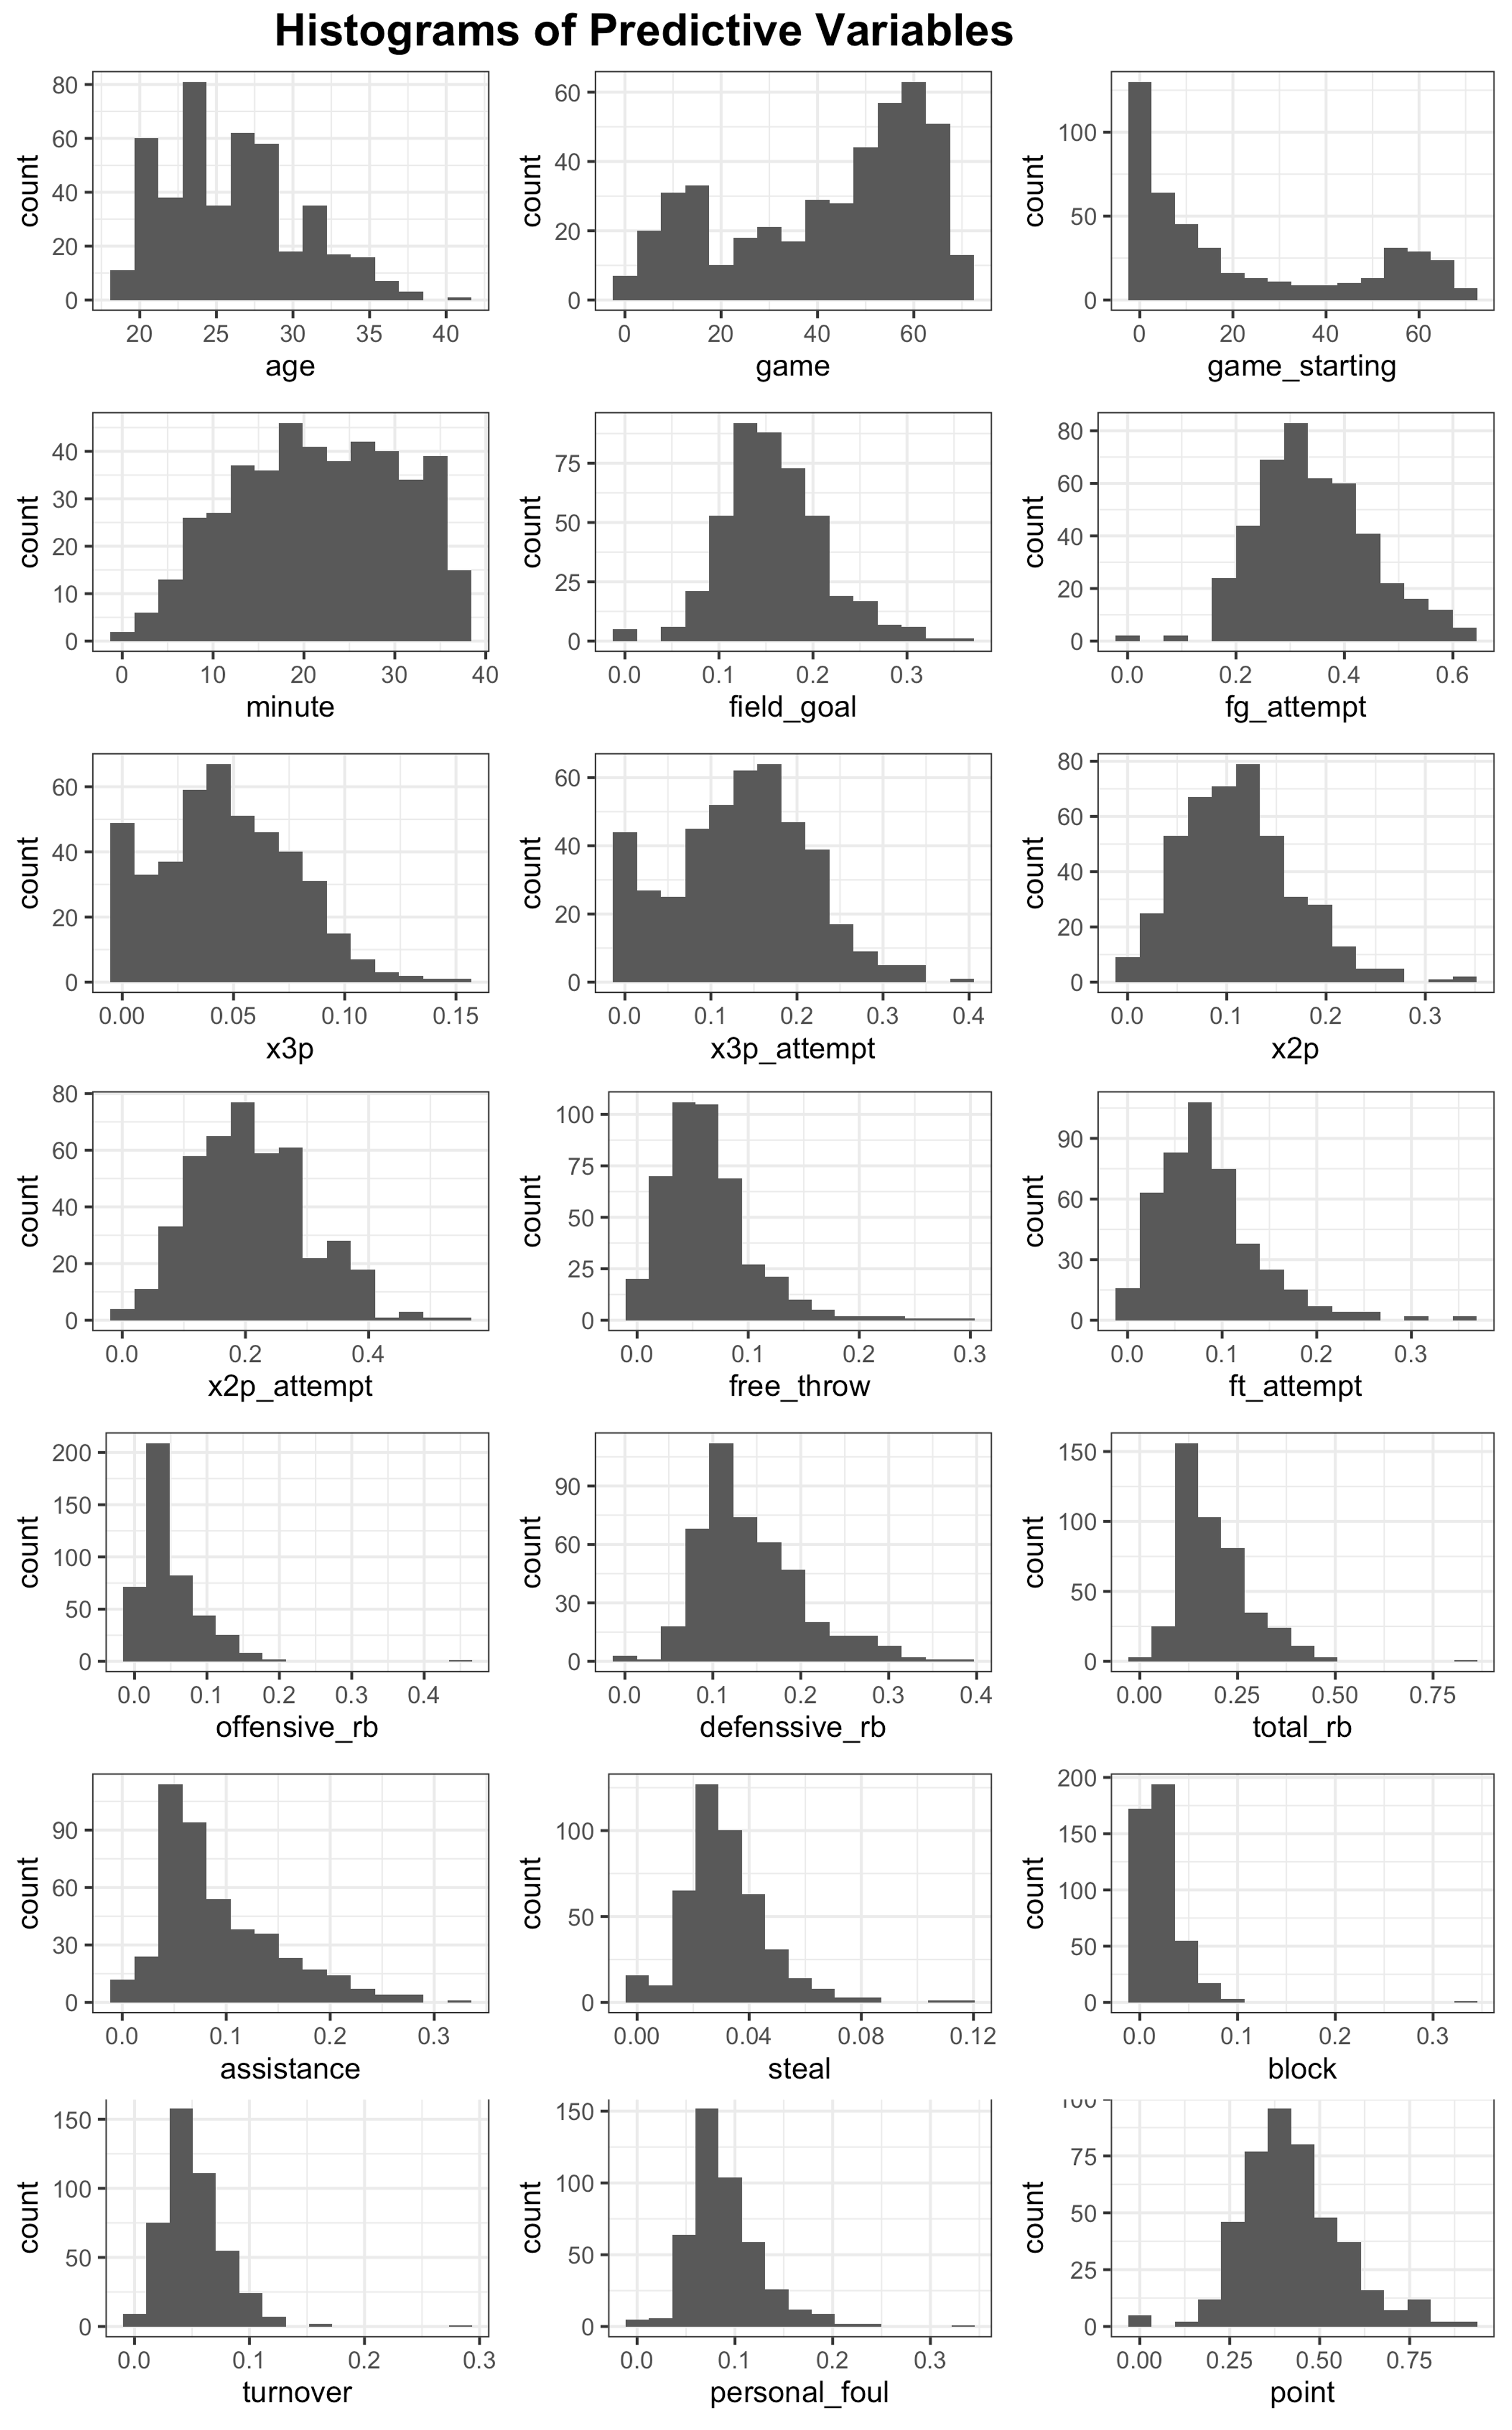
\includegraphics[width=\textwidth,height=0.8\textheight]{report_figures/appendixA_figure01.png}
\caption{Histograms of Predictive Variables}
\end{figure}

\newpage

\begin{figure}
\centering
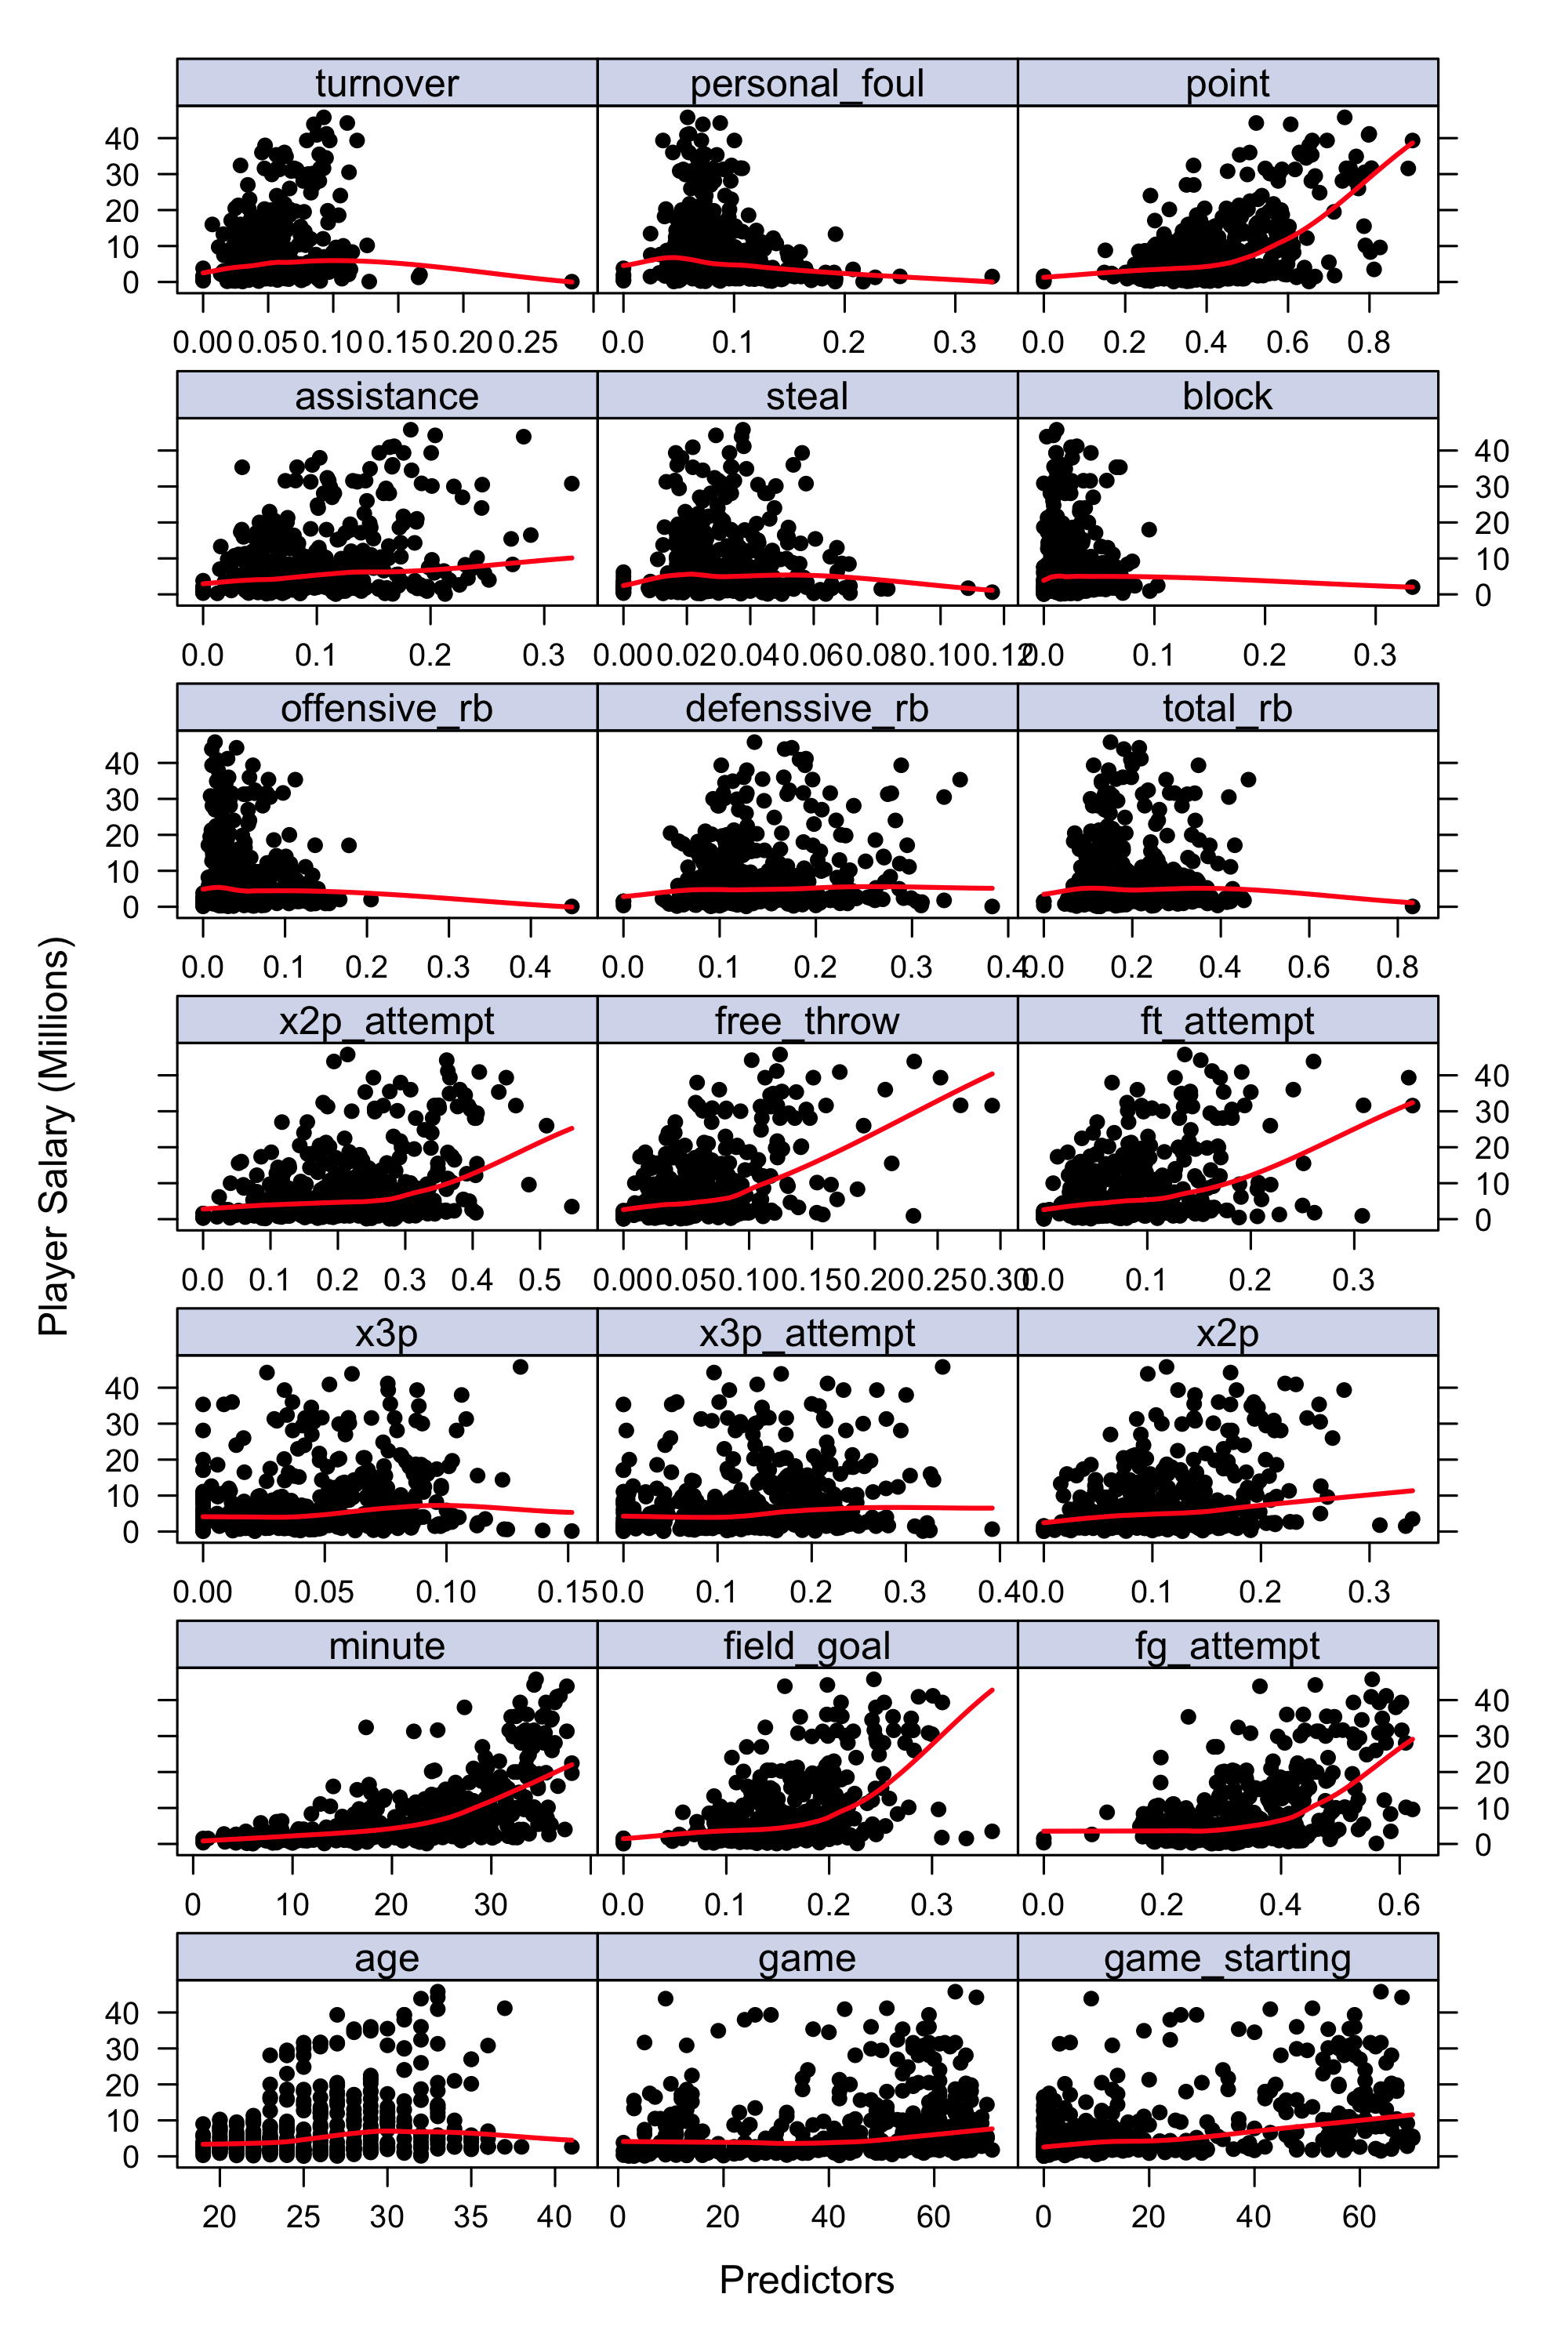
\includegraphics[width=\textwidth,height=0.7\textheight]{report_figures/appendixA_figure4.png}
\caption{Featureplot of Numeric Variables}
\end{figure}

\newpage

\hypertarget{appendix-b---linear-regerssion}{%
\subsubsection{Appendix B - Linear
Regerssion}\label{appendix-b---linear-regerssion}}

\begin{figure}
\centering
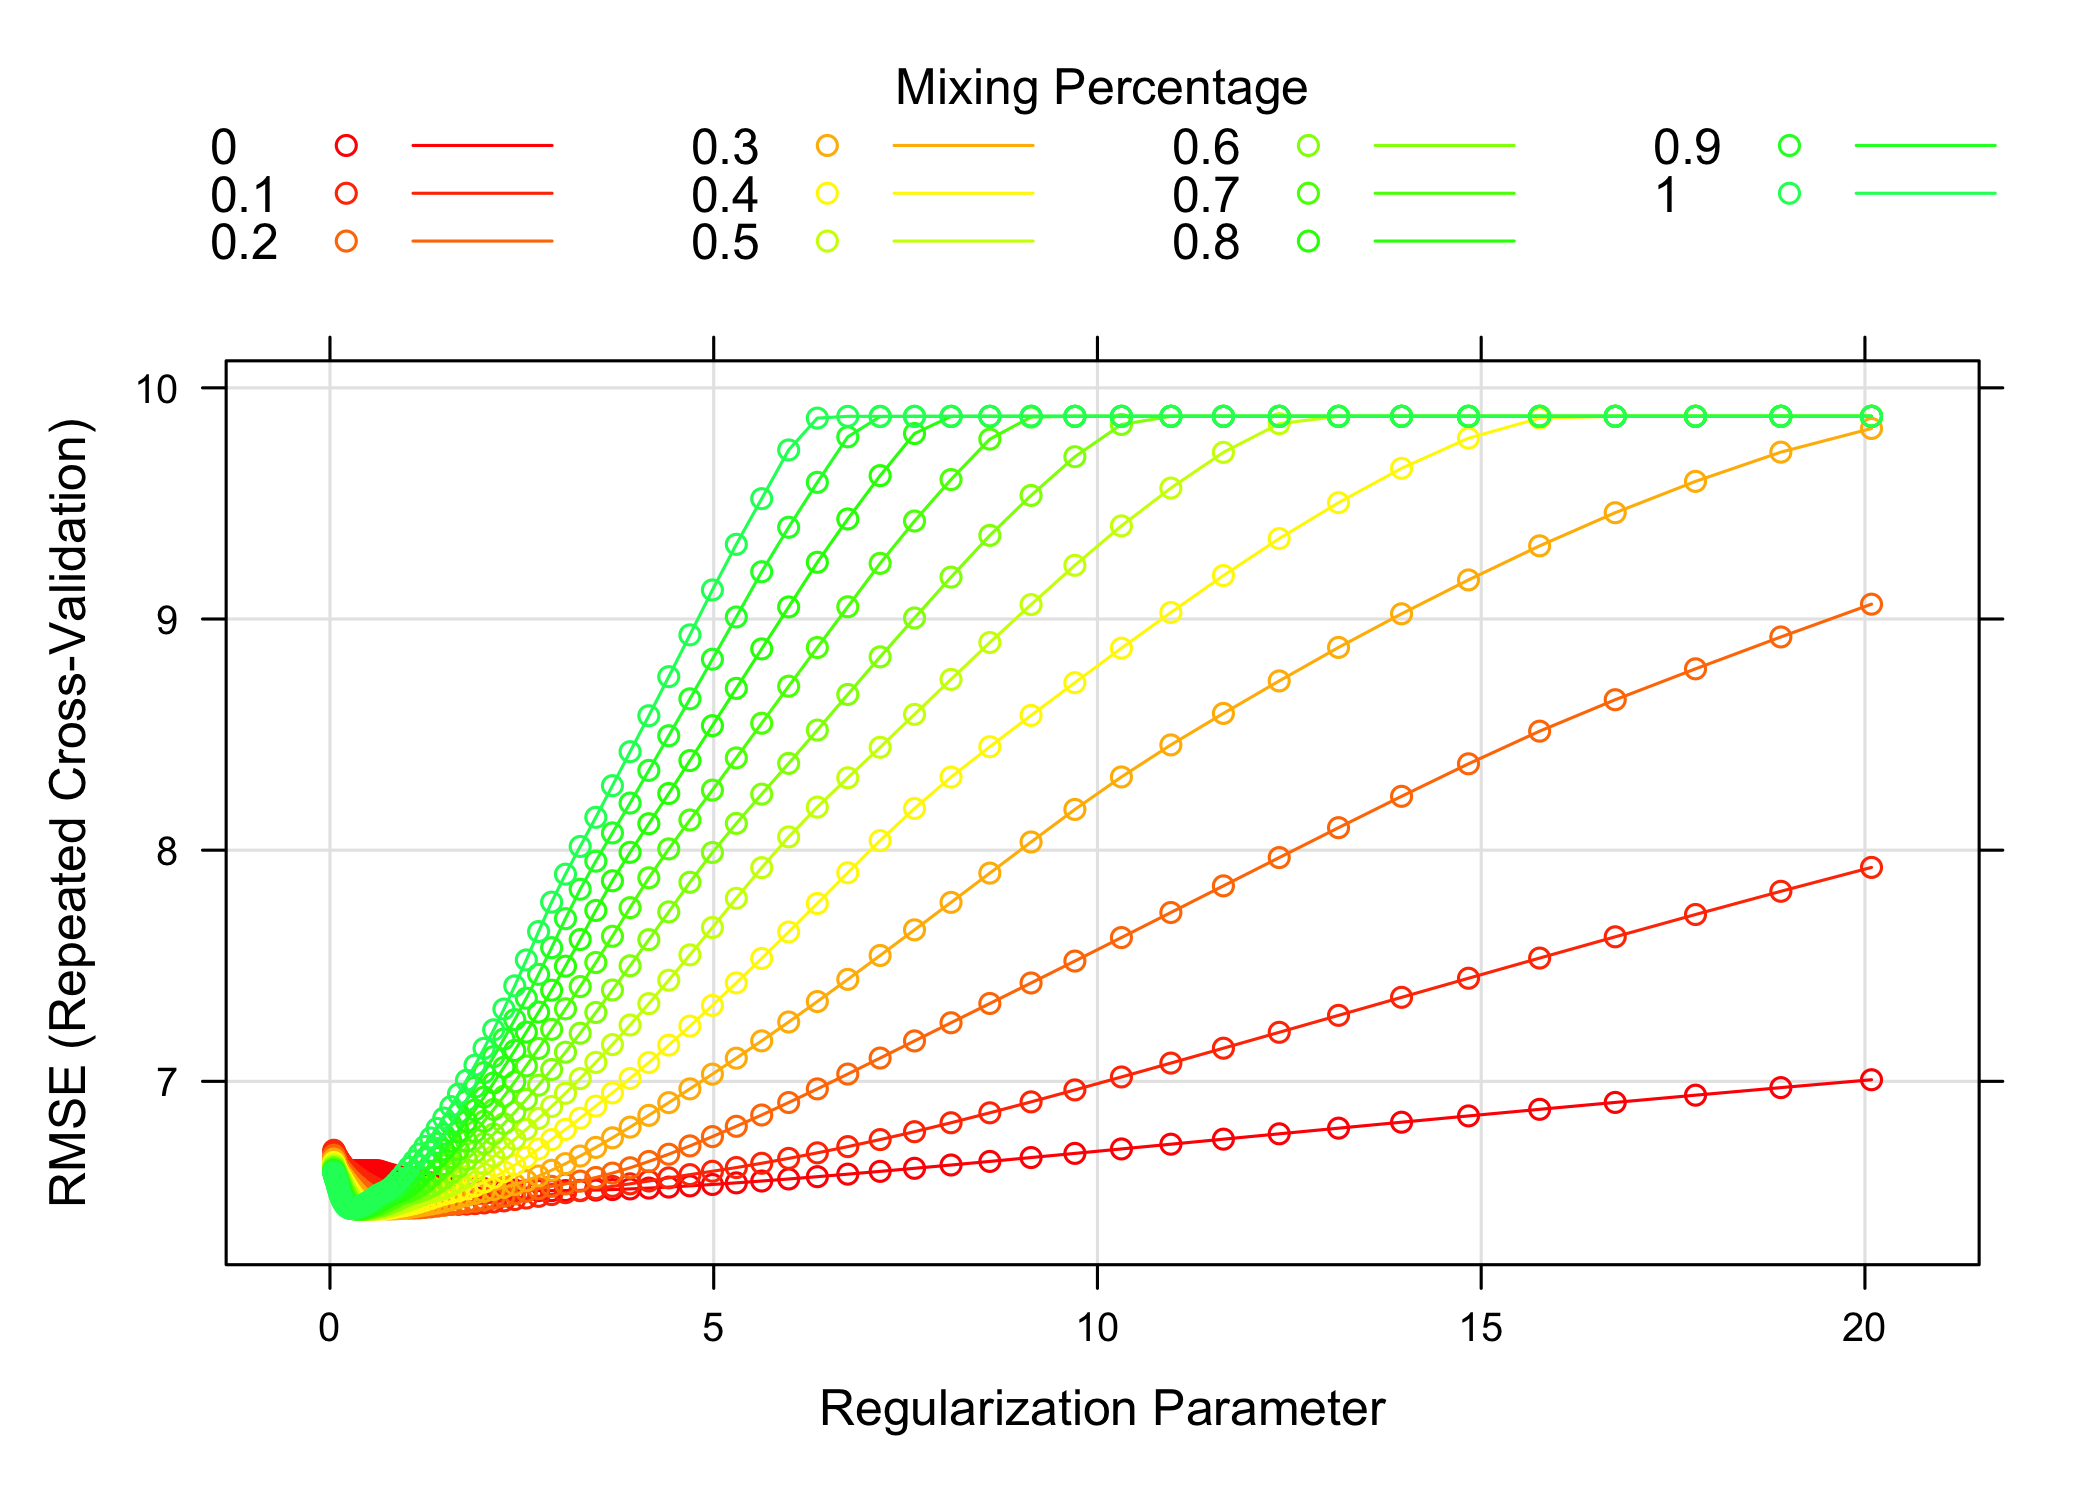
\includegraphics{report_figures/appendixB_figure1.png}
\caption{Parameter Tuning Plot of Elastic-net Model}
\end{figure}

\begin{figure}
\centering
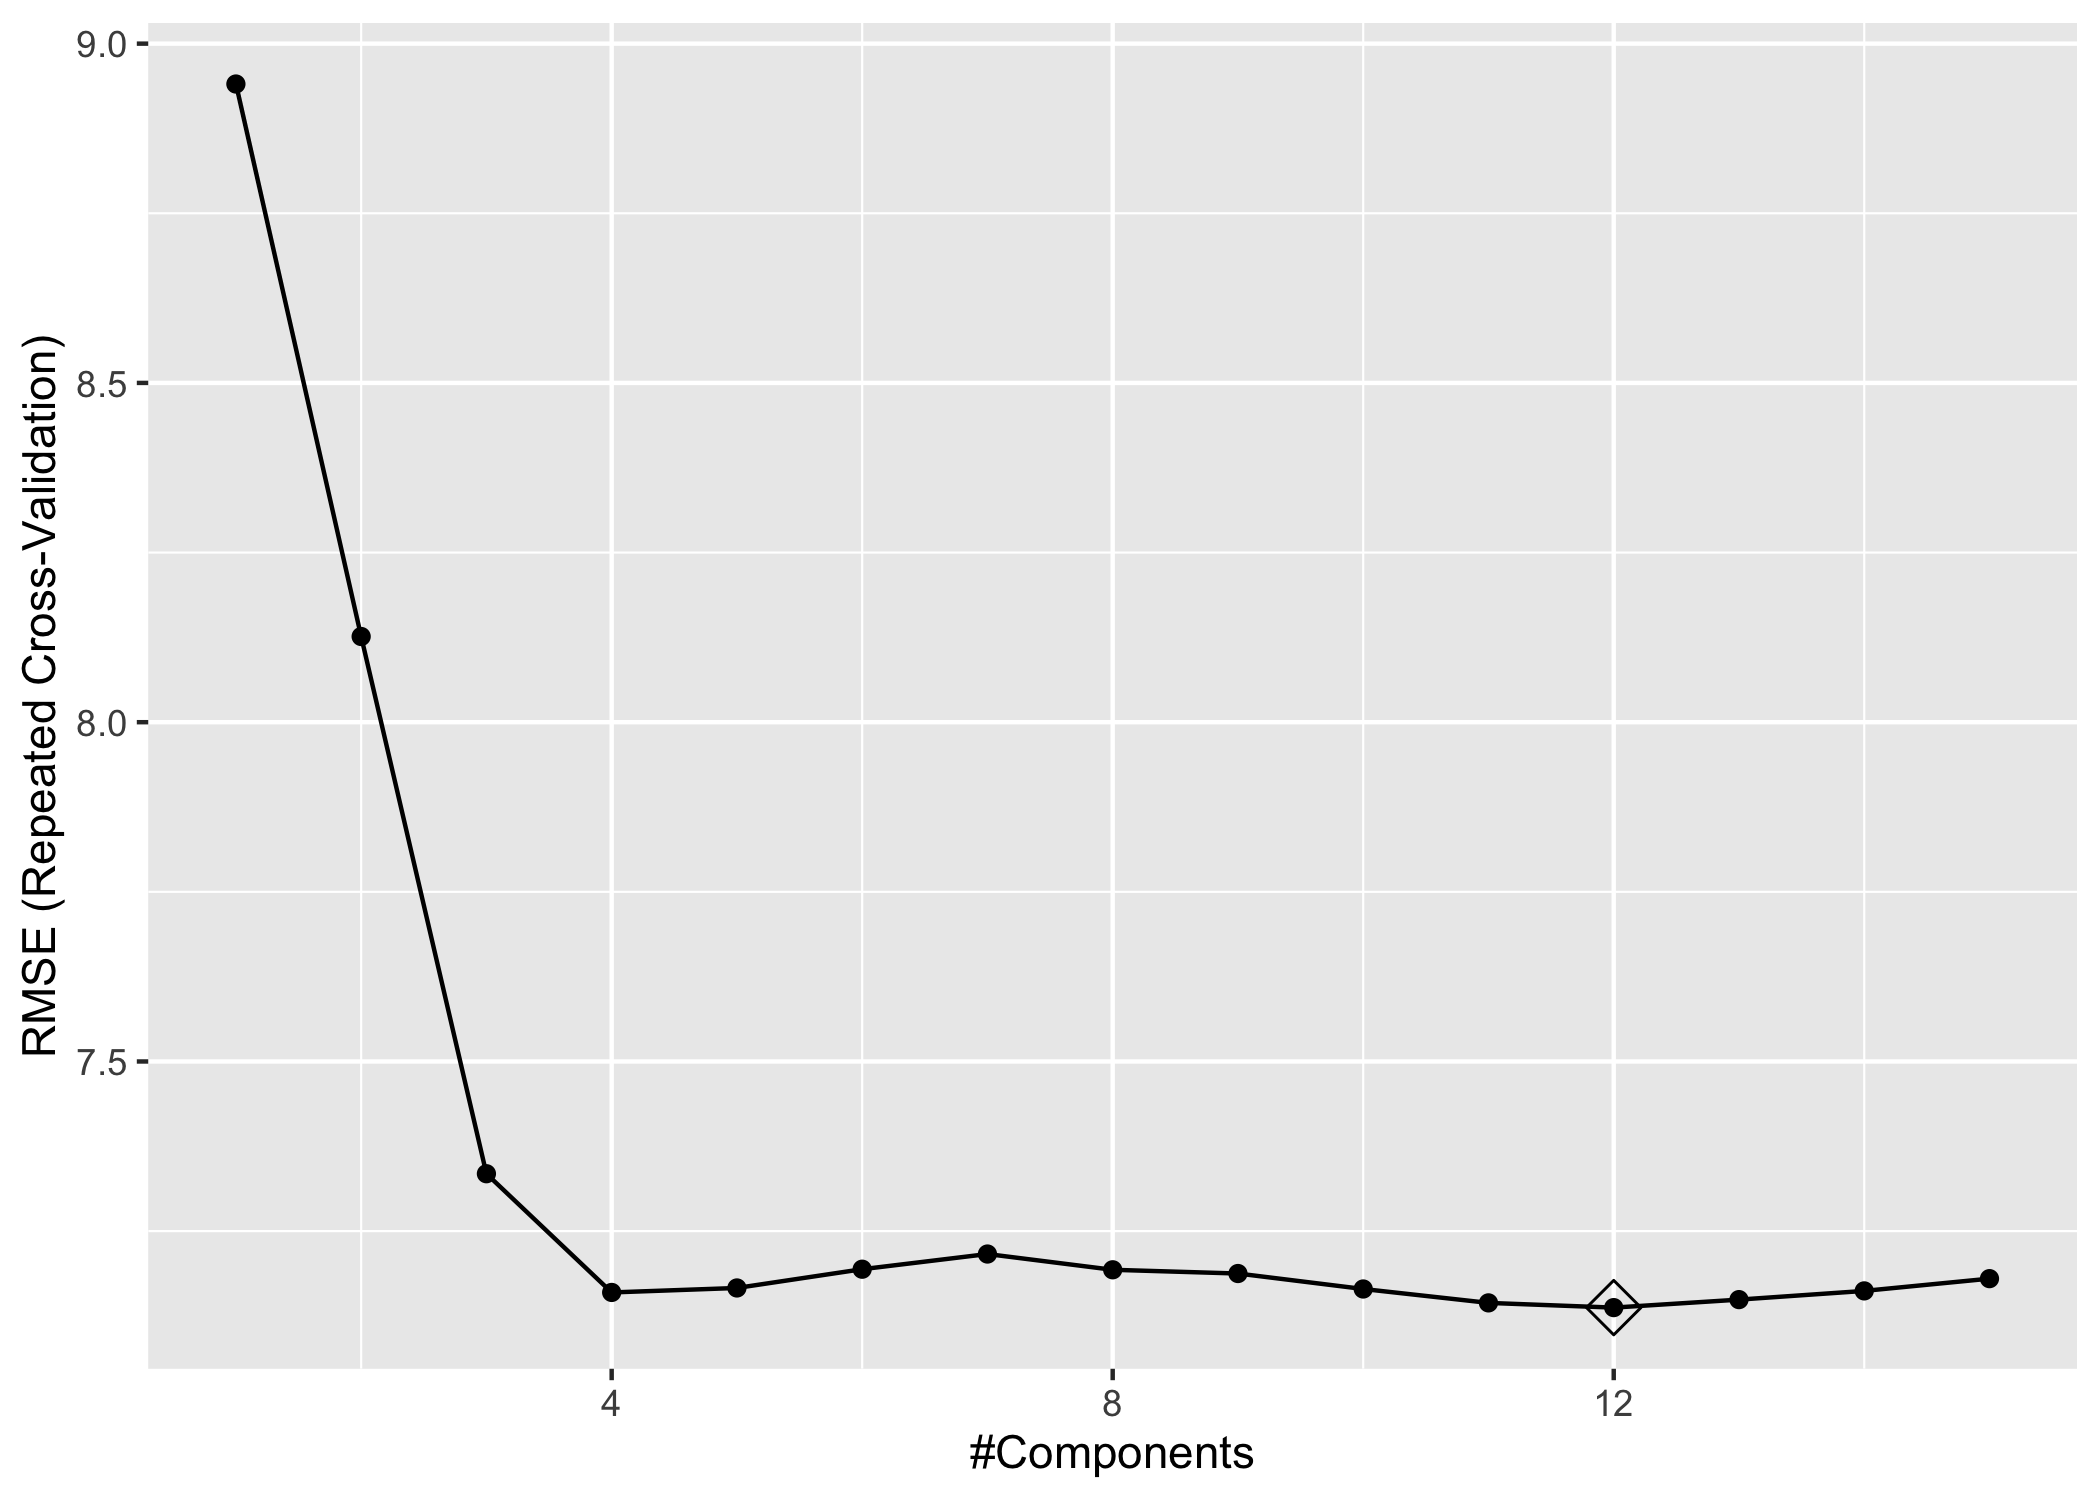
\includegraphics{report_figures/appendixB_figure2.png}
\caption{Parameter Tuning of PCR}
\end{figure}

\begin{figure}
\centering
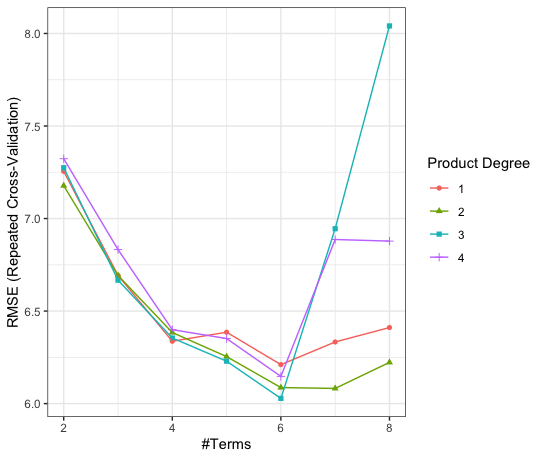
\includegraphics{report_figures/appendixB_figure3.png}
\caption{Parameter Tuning of MARS}
\end{figure}

\newpage

\hypertarget{appendix-c---tree-based-models}{%
\subsubsection{Appendix C - Tree-based
Models}\label{appendix-c---tree-based-models}}

\begin{figure}
\centering
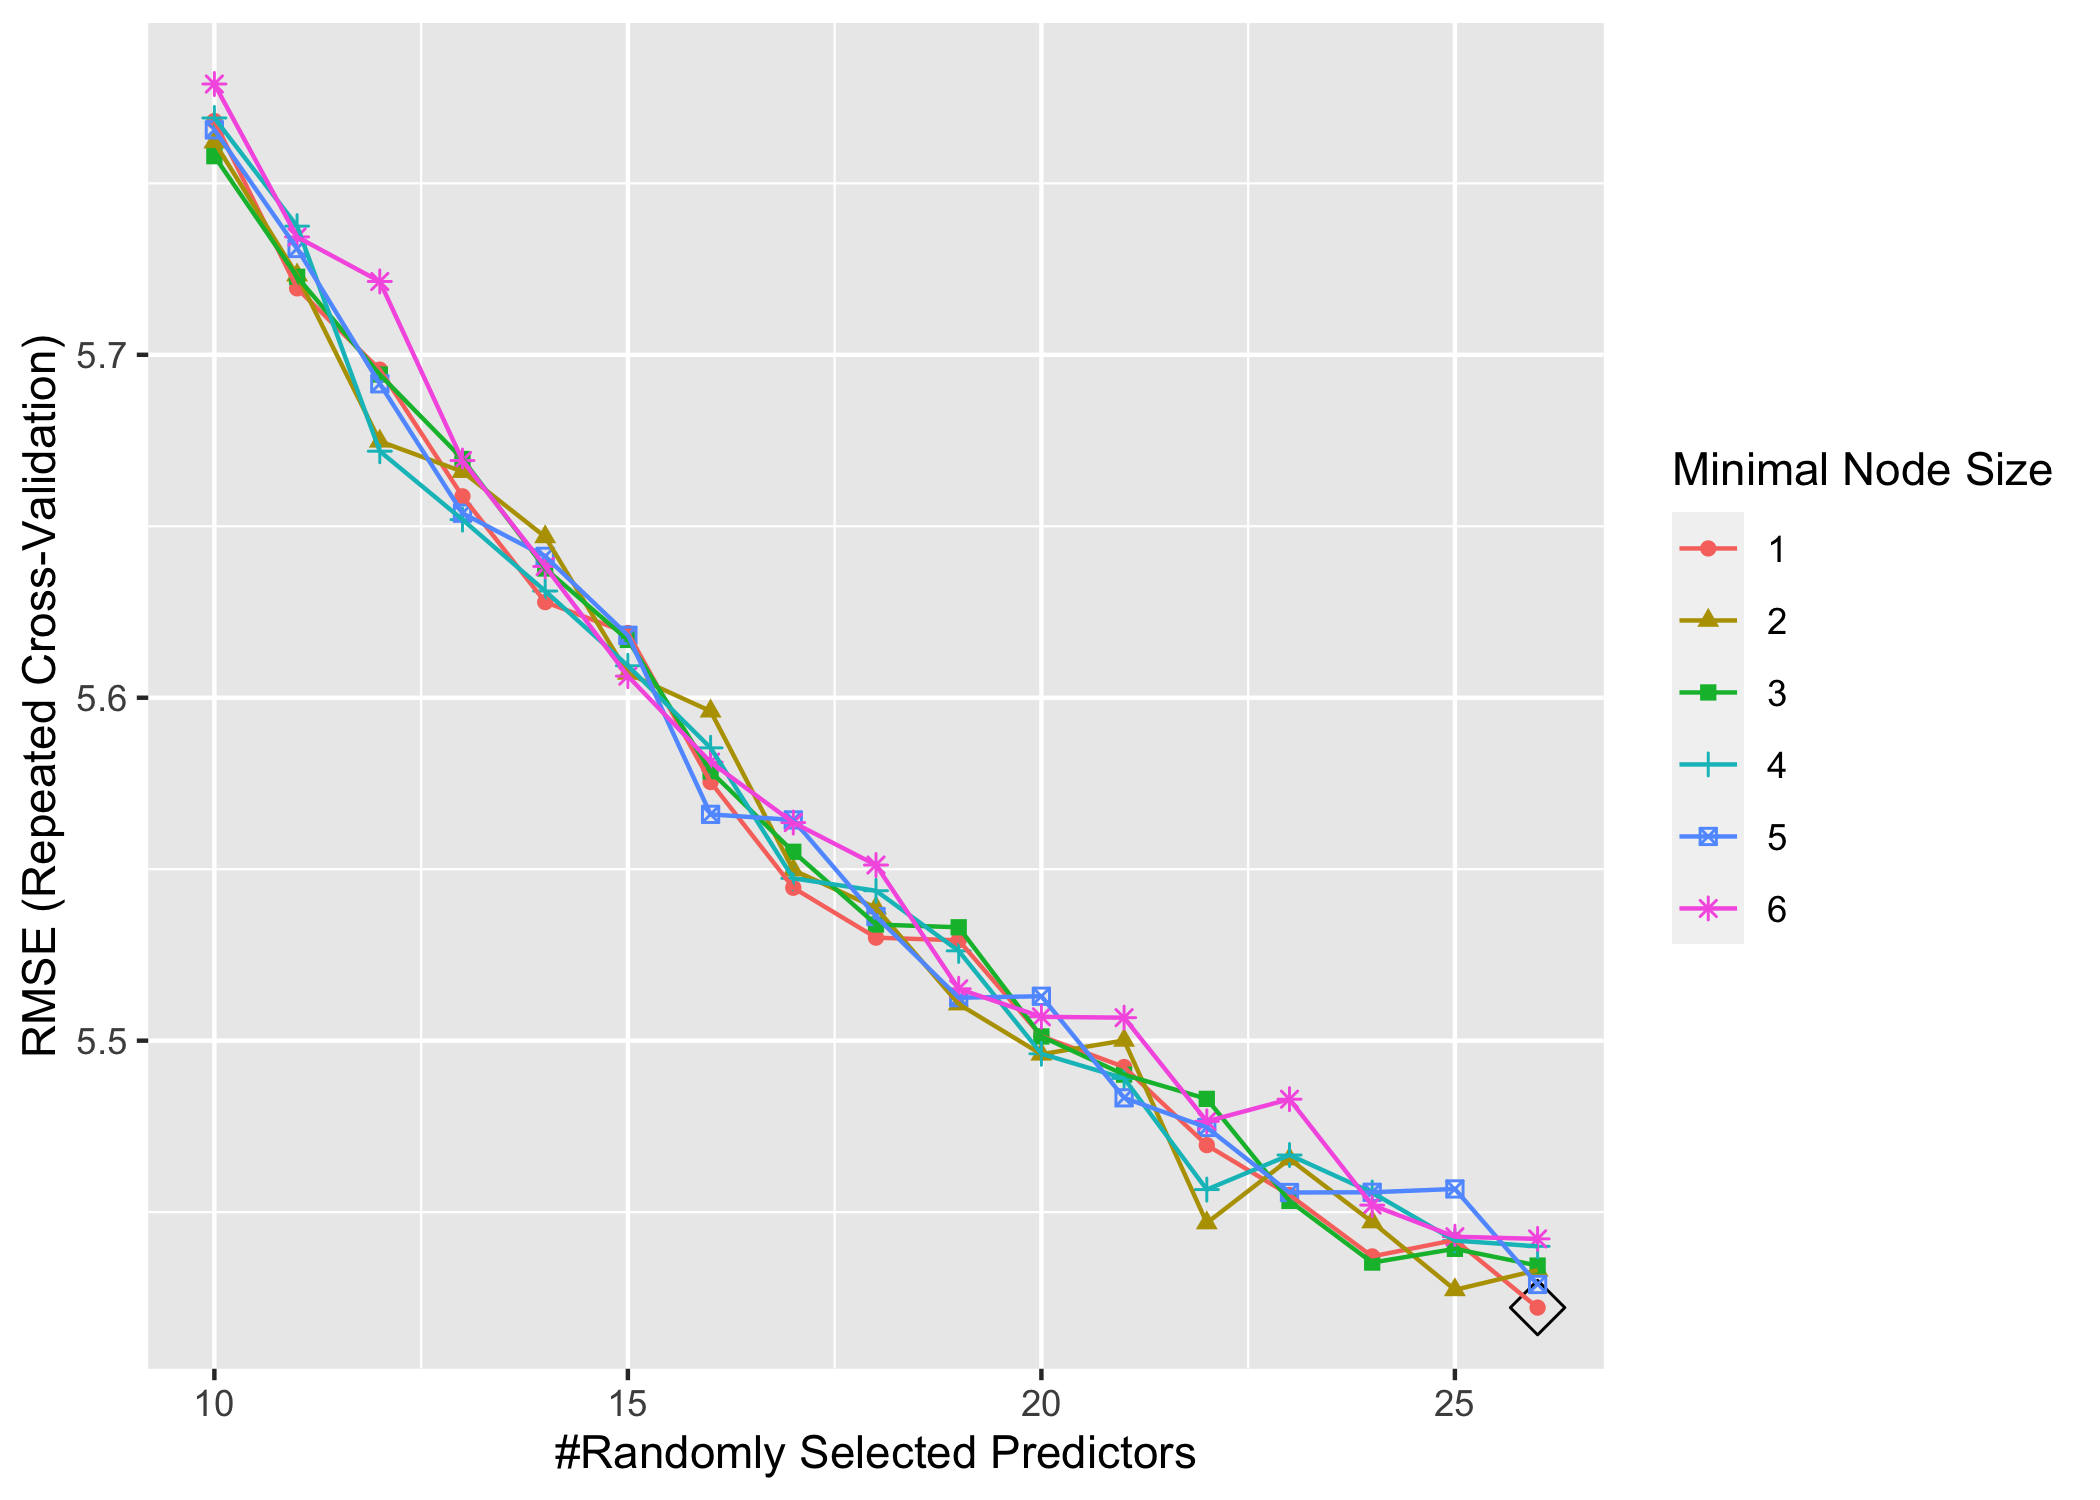
\includegraphics{report_figures/appendixC_figure2.png}
\caption{Parameter Tuning of Random Forest}
\end{figure}

\begin{figure}
\centering
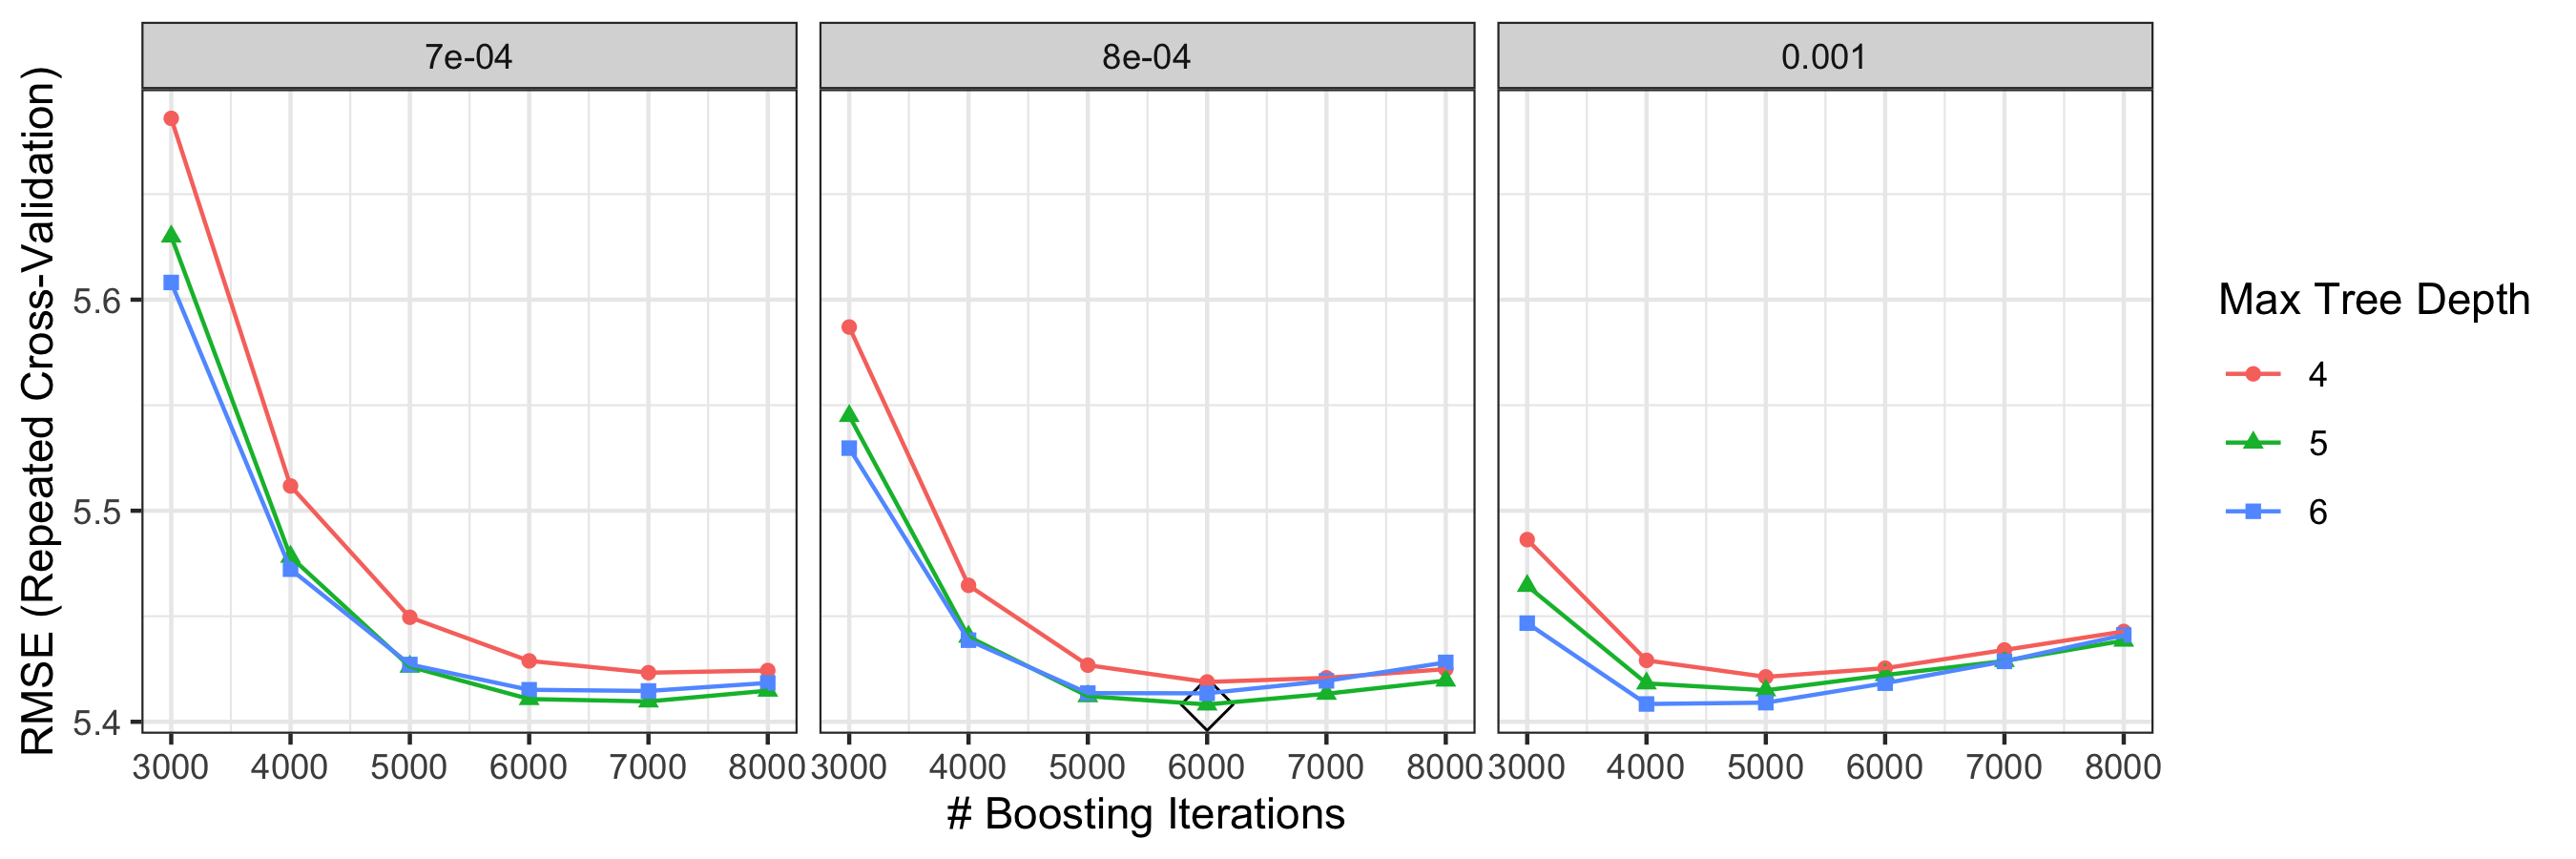
\includegraphics{report_figures/appendixC_figure1.png}
\caption{Parameter Tuning of of GBM}
\end{figure}

\end{document}
